\chapter{Background processes}
\label{chap:backgrounds}

Two classes of background processes are present in this search: reducible and irreducible. For the former category, a particle in the background process may ``fake'' the signature of a particle that is expected in the signal process. On the contrary, in the case of the latter category, the final state topology of the background process yields the same expected particles as a potential signal process. A key feature of reducible backgrounds is the ability to suppress such processes by employing the selection cuts as described in Sec.~\ref{sec:selection}. Furthermore, some of the reducible background contributions are estimated using data-driven techniques. In large part, however, the dominant backgrounds in the search are estimated from simulations.

Sec.~\ref{sec:tt2l}-\ref{sec:fakes} describe the relevant SM backgrounds in the search for \ttllDM. The production cross sections at $\sqrt{s}=13\:\TeV$ for these backgrounds are shown in~\FigureRef{fig:SMxsec}, giving a sense of the relative importance of the processes. The phase space targeted by the selection requirements as described in Sec.~\ref{sec:selection} also affects the relative hierarchy of the backgrounds, though it remains true that processes with larger cross sections, such as \ttbar and Drell-Yan, are dominant in the regions of highest sensitivity.

\begin{figure}
  \begin{center}
    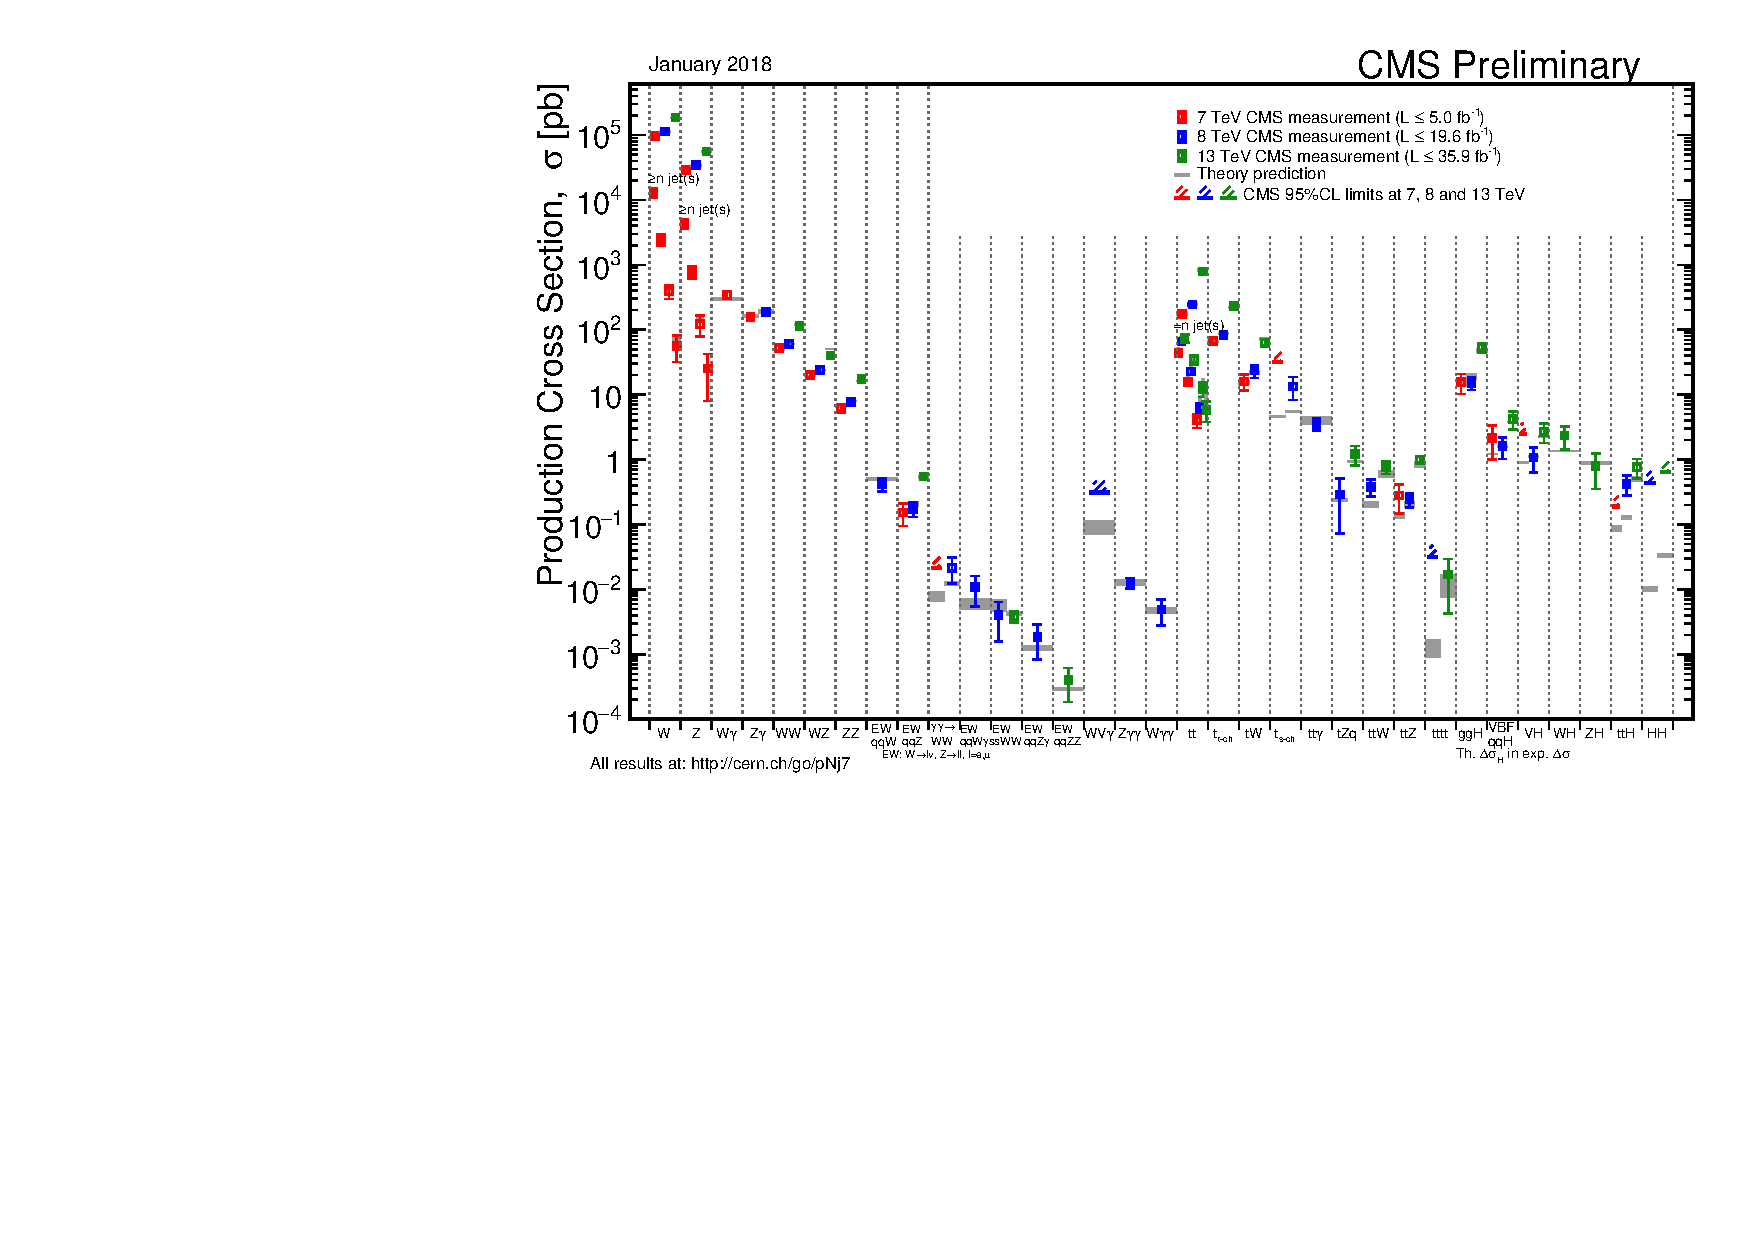
\includegraphics[width=\textwidth]{figs/SigmaNew_v0.pdf}
    \caption{Summary of the cross section measurements of SM processes as of January 2018 with data collected by the CMS experiment at $\sqrt{s}=7,\:8,\:\text{and}\: 13\:\TeV$. }
    \label{fig:SMxsec}
  \end{center}
\end{figure}

\begin{figure}
  \begin{center}
    \subfloat[][]{\label{fig:gg_tt}
      \feynmandiagram[horizontal=b to c]{
        a [particle=\(g\)] -- [gluon] b -- [gluon] c,
        d [particle=\(g\)] -- [gluon] b,
        e [particle=\(\bar{t}\)] -- [fermion] c,
        c -- [fermion] f [particle=\(t\)],
      };
    }
    \hspace{0.5cm}
    \subfloat[][]{\label{fig:gg_tt2}
      \feynmandiagram[vertical=b to d]{
        a [particle=\(g\)] -- [gluon] b,
        c [particle=\(\bar{t}\)] -- [fermion] b -- [fermion] d -- [fermion] f [particle=\(t\)], 
        e [particle=\(g\)] -- [gluon] d,
        a -- [opacity=0.0001] e,
        c -- [opacity=0.0001] f,
      };
    }
    \hspace{0.5cm}
    \subfloat[][]{\label{fig:qq_tt}
      \feynmandiagram[horizontal=b to d]{
        a [particle=\(q\)] -- [fermion] b -- [fermion] c [particle=\(\bar{q}\)],
        b -- [gluon] d,
        f [particle=\(\bar{t}\)] -- [fermion] d -- [fermion] e [particle=\(t\)],
      };
    }
  \end{center}
  \caption{Leading order \ttbar production diagrams probed at the LHC via~\protect\subref{fig:gg_tt},~\protect\subref{fig:gg_tt2} gluon fusion, and~\protect\subref{fig:qq_tt} quark-antiquark annihilation.}
\label{fig:tt2l_feyn}
\end{figure}
%%------------------------- tt2l -------------------------%%  
\section{\ttll}
\label{sec:tt2l}
SM \ttll is the dominant background contribution and is irreducible, owing to the similarity of the final state topology with the signal processes topology. At the LHC, approximately 90\% of \ttbar events are produced via gluon fusion as shown in~\FigureRef{fig:gg_tt} and ~\FigureRef{fig:gg_tt2}, in contrast to the Tevatron at Fermilab, where quark-antiquark annihilation shown in~\FigureRef{fig:qq_tt} constituted roughly 85-90\% of the relative \ttbar production. 

The theoretical uncertainties incurred at leading order (LO) in perturbative QCD are quite large for \ttbar production. In addition to the LO simulation, the \ttbar process decaying to the dilepton final state is simulated at next-to-leading order (NLO) using the \POWHEG \textsc{v2}~\cite{powheg,powheg2} generator, with the top quark mass assumed to be \mtop=172.5\:\GeV. These events are then interfaced to \Pythia \textsc{v8.2}~\cite{Sjostrand:2014zea} for parton fragmentation, hadronization, and to simulate the underlying event. As pertains to all simulated samples subsequently described, once the \ttll events are showered, the detector response is simulated using the \Geant 4 program~\cite{AGOSTINELLI2003250}. Finally, the \ttll events are normalized to the theoretical cross section calculated at next-to-next-to-leading order (NNLO) in perturbative QCD, which also includes soft-gluon resummation calculations at next-to-next-to-leading-order (NNLL)~\cite{ttxsec1,ttxsec2,ttxsec3,ttxsec4,ttxsec5}. The cross-section folds in the branching fraction of \ttbar to the dilepton final state, which is 10.5\%. The cross-section value used is $\sigma_{\ttll}=87.31\:\mathrm{pb}$.

As mentioned in Sec.~\ref{subsec:mt2ll}, the \ttll background should be suppressed below the kinematic endpoint, $M_W$, in the \mttll distribution. This would only be possible in ideal measurement conditions, however as a cause of detector and energy resolution effects, the mismeasurement of the objects in \ttll background events can contribute to values of \mttll$>\:M_W$. 

%%------------------------- ttV,VV,ST -------------------------%%  
\section{\ttV, diboson, and single top processes}
\label{sec:ttVetc}
Among the more rare processes considered as backgrounds to this search are processes wherein a top quark pair is produced in association with a boson, denoted as \ttV (where V=\gamma, Z, W). In particular for the $\mathrm{t\bar{t}}$+Z process, as shown in~\FigureRef{fig:ttV}, the same final state is expected as the signal so this process falls under the class of irreducible backgrounds. Although the production cross-sections for \ttV processes are orders of magnitude smaller than the \ttbar production cross-section, this background is significant in the high \mttll categories. The moderate \ptmiss requirement is inefficient in \ttV background reduction, since large values of \ptmiss are expected. In addition, the $\mathrm{t\bar{t}}$+Z process will leak into the high \mttll category as a cause of the additional expected \ptmiss from the neutrinos, which bias the minimization over all the two-way partitions of the \ptmiss, resulting in high values of \mttll.

The diboson background processes encompass WW, ZZ, and WZ production where all possible final states (i.e. decays to $q\bar{q}$, $\ell\nu$, $\ell\ell$, and $\nu_\ell\bar{\nu}_\ell$) are considered for the relevant boson. Owing in part to the largest relative production cross-section, the WW process is the dominant diboson process. In particular, the dilepton signal region requirement targets the final state where both W bosons decay to lepton-neutrino pairs. 
 
The single top background is also expected to contribute sub-dominantly in the signal region. The lepton multiplicity requirement serves to suppress the contributions from s- and t-channel production (i.e. processes whose amplitudes go as $\mathscr{M}\sim 1/s$ and $\mathscr{M}\sim 1/t$, where $s$ and $t$ correspond to the Mandelstam variables), as seen in~\FigureRef{fig:s-channel} and~\FigureRef{fig:t-channel}, since only one prompt lepton is expected. Thus, the dilepton final state tW associated production diagram, shown in~\FigureRef{fig:tW}, contributes the most significantly to the single top background.  

Similarly to the \ttll process, the \ttV, diboson, and single top processes are simulated at NLO. The \ttV processes are generated using \AMCATNLO \textsc{v2.2.2}. For single top, the s- and t-channel processes are simulated using \POWHEG \textsc{v2} and interfaced with \MadSpin which decays the top and preserves the spin correlation and any finite width effects in narrow resonance decays. The tW channel, on the other hand, is generated using \POWHEG \textsc{v1} at NLO accuracy and normalized to the approximate NNLO cross-section. The diboson samples are generated at NLO using either \AMCATNLO \textsc{v2.2.2} or \POWHEG \textsc{v2}.
 
\begin{figure}
  \begin{center}
    \subfloat[][\ttV]{\label{fig:ttV}
      \feynmandiagram[vertical=c to b] {
        a [particle=\(q\)] -- [fermion] b -- [fermion] c -- [fermion] d [particle=\(\bar{q}\)],
        b -- [boson, edge label=\(Z\)] e,
        i [particle=\(\bar{\nu}_\ell\)] -- [fermion] e -- [fermion] j [particle=\(\nu_\ell\)],
        c -- [gluon, edge label'=\(g\)] f,
        g [particle=\(\bar{t}\)] -- [fermion] f -- [fermion] h [particle=\(t\)],
%        f -- [opacity=0.0001] e,
%        a -- [opacity=0.0001] d,
      };
    }
    \hspace{1cm}
    \subfloat[][Diboson]{\label{fig:VV}
      \feynmandiagram[vertical=b to c] {
        a [particle=\(q\)] -- [fermion] b -- [fermion] c -- [fermion] d [particle=\(\bar{q}\)],
        b -- [boson] f [particle=\(V\)],
        c -- [boson] e [particle=\(V\)],
        a -- [opacity=0.0001] d,
%        f -- [opacity=0.0001] e,
      };
    }
    \caption{Examples of the~\protect\subref{fig:ttV} \ttV process, and ~\protect\subref{fig:VV} diboson production at LO.}
    \label{fig:diboson_feyn}
  \end{center}
\end{figure}

\begin{figure}
  \begin{center}
    \subfloat[][s-channel]{\label{fig:s-channel}
      \feynmandiagram[horizontal=b to e]{
        a [particle=\(u\)] -- [fermion] b -- [fermion] c [particle=\(d\)],
        d [particle=\(b\)] -- [fermion] e -- [fermion] f [particle=\(t\)],
        b -- [boson, edge label' = \(W^+\)] e,
      };
    }
    \hspace{0.5cm}
    \subfloat[][t-channel]{\label{fig:t-channel}
      \feynmandiagram[vertical=b to e]{
        a [particle=\(u\)] -- [fermion] b -- [fermion] c [particle=\(d\)],
        d [particle=\(b\)] -- [fermion] e -- [fermion] f [particle=\(t\)],
        b -- [boson, edge label = \(W^+\)] e,    
      };
    }
    \hspace{0.5cm}
    \subfloat[][tW-associated]{\label{fig:tW}
      \feynmandiagram[horizontal=b to c]{
        a [particle=\(b\)] -- [fermion] b -- [fermion, edge label=\(b\)] c -- [fermion] d [particle=\(t\)],
        e [particle=\(g\)] -- [gluon] b,
        c -- [boson] f [particle=\(W^-\)], 
      };
    }
    \caption{Single top quark production via~\protect\subref{fig:s-channel} s-channel,~\protect\subref{fig:t-channel} t-channel, and~\protect\subref{fig:tW} in association with a W boson.}
    \label{fig:st_feyn}
  \end{center}
\end{figure}

%%------------------------- DY -------------------------%%  
\section{Drell-Yan}
\label{sec:DY}
\begin{figure}
  \begin{center}
    \subfloat[][]{\label{fig:dy1}
      \feynmandiagram[horizontal=b to d]{
        a [particle=\(q\)] -- [fermion] b -- [fermion] c [particle=\(\bar{q}\)],
        f [particle=\(\ell^{+}\)] -- [fermion] d -- [fermion] e [particle=\(\ell^{-}\)], 
        b -- [boson, edge label=\(\gamma^{*}/Z\)] d,
      };
    } 
    \subfloat[][]{\label{fig:dy2}
      \feynmandiagram[horizontal=b to c] {
        a [particle=\(q\)] -- [fermion] b -- [fermion] c -- [fermion] d [particle=\(q\)],
        e [particle=\(g\)] -- [gluon] b,
        c -- [boson, edge label=\(\gamma^{*}/Z\)] g,
        h [particle=\(\ell^{+}\)] -- [fermion] g -- [fermion] f [particle=\(\ell^{-}\)], 
        d -- [opacity=0.0001] f,
      };
    }  
    \subfloat[][]{\label{fig:dy3}
      \feynmandiagram[vertical=b to c] {
        a [particle=\(q\)] -- [fermion] b -- [fermion] c -- [fermion] d [particle=\(q\)],
        e [particle=\(g\)] -- [gluon] c,
        b -- [boson, edge label=\(\gamma^{*}/Z\)] g,
        h [particle=\(\ell^{+}\)] -- [fermion] g -- [fermion] f [particle=\(\ell^{-}\)], 
        d -- [opacity=0.0001] h,
      }; 
    } \\
    \subfloat[][]{\label{fig:dy4}
      \feynmandiagram[horizontal=b to g] {
        a [particle=\(q\)] -- [fermion] b -- [fermion] c -- [fermion] d [particle=\(\bar{q}\)],
        e [particle=\(g\)] -- [gluon] c,
        b -- [boson, edge label=\(\gamma^{*}/Z\)] g,
        h [particle=\(\ell^{+}\)] -- [fermion] g -- [fermion] f [particle=\(\ell^{-}\)], 
        e -- [opacity=0.0001] h,
      };
    } 
    \hspace{0.7cm}
    \subfloat[][]{\label{fig:dy5}
      \feynmandiagram[vertical=b to c] {
        a [particle=\(q\)] -- [fermion] b -- [fermion] c -- [fermion] d [particle=\(\bar{q}\)],
        e [particle=\(g\)] -- [gluon] b,
        c -- [boson, edge label=\(\gamma^{*}/Z\)] g,
        h [particle=\(\ell^{+}\)] -- [fermion] g -- [fermion] f [particle=\(\ell^{-}\)], 
        e -- [opacity=0.0001] f,
      };
    }
  \end{center}
  \caption{The Drell-Yan lepton pair-production process mediated by a virtual photon ($\gamma^{*}$) or Z boson at~\protect\subref{fig:dy1} $\mathcal{O}$($\alpha$) and~\protect\subref{fig:dy2},\protect\subref{fig:dy3},\protect\subref{fig:dy4},\protect\subref{fig:dy5} $\mathcal{O}$($\alpha\alpha_{s}$).}
  \label{fig:dy_feyn}
\end{figure}

From the diagrams in~\FigureRef{fig:dy_feyn}, the Drell-Yan pair-production process falls under the class of reducible backgrounds, since many of the selection criteria act to suppress processes where the selected same flavor opposite sign (SFOS) leptons are produced at the same vertex, such as from the exchange of a real Z boson or a virtual photon ($\gamma^{*}$). Namely, the requirement for the mass of the selected SFOS lepton pair to be outside of the Z mass window, 75\:\GeV$< M_{Z} <$105\:\GeV, removes a large contribution of dilepton decays stemming from real Z bosons/off-shell virtual photons. Furthermore, the low dilepton mass requirement, $M_{\ell\ell}>20\:\GeV$ suppresses the contribution from low mass decays of $J/$\psi mesons to SFOS pairs. In addition, the requirement for the event to contain at least two jets, with at least one b-tagged jet acts to eliminate contributions from~\FigureRef{fig:dy1}, where the quark-antiquark annihilation to a SFOS pair proceeds at LO in $\alpha$. The DY process is simulated at NLO using \AMCATNLO \textsc{v2.3.3}, and thus includes contributions from higher order processes as shown in~\FigureRef{fig:dy2}-\FigureRef{fig:dy5}, where at least one jet is expected from the fragmentation and hadronization of particles emmitted in initial state radiation.

Although the relative shape of the DY contribution is taken from simulation, a data-driven process is used to estimate the normalization of this background. The signal region still contains a size-able DY contribution, meaning that exceptional DY events evading the above-mentioned Z boson mass veto tend to be accompanied by a significant amount of \ptmiss. Since the instrumental detector effects which influence this final state topology are non-trivial to simulate, it is more appropriate to use calibrated samples from data to arrive at these estimates.  

\subsection{The \Rinout method}

The method is used to predict the DY normalization, $N_{DY}$, by extrapolating from the observed DY yield inside the Z mass window (within $\pm15\:\GeV$ of $M_{Z}$), $N_{in}$, according to:

\begin{equation}
  N_{DY} = N_{in}\frac{R^{0b}_{\mathrm{MC}}}{R^{1b}_{\mathrm{MC}}\cdot R^{0b}_{\mathrm{data}}},
  \label{eq:NDY}
\end{equation}

where each quantity $R$ in Eq.~\ref{eq:NDY} is defined as the ratio of DY yields \textbf{in}side to \textbf{out}side the Z mass window, 

\begin{equation}
  \Rinout = \frac{N(|M_{\ell\ell} - M_Z|<15\:\GeV)}{N(|M_{\ell\ell} - M_Z|>15\:\GeV\mbox{ and }M_{\ell\ell}>20\:\GeV)}.
  \label{eq:Rinout}
\end{equation}

Hence, the events originally rejected by the Z veto are used to estimate the residual contributions from DY $\rightarrow e^+e^-$ and $\mu^+\mu^-$ in the remaining selected sample. The yields are computed with all other selection cuts applied. Ideally, the \Rinout in a region where the number of b-tagged jets is required to be zero would be equal to the \Rinout in a region where at least one b-tagged jet is required, such that $\Rinout^{0b} = \Rinout^{1b}$. This assumption, however, is invalid since the numerator and denominator in Eq.~\ref{eq:Rinout} differ significantly when measured in DY simulation with a looser set of selection cuts, such as the removal of the \ptmiss requirement or a looser jet multiplicity requirement. A weaker assumption is then made, which is as follows:

\begin{equation}
  \frac{\left(\Rinout^{1b}\right)_{\mbox{data}}}{\left(\Rinout^{1b}\right)_{\mbox{MC}}} = 
  \frac{\left(\Rinout^{0b}\right)_{\mbox{data}}}{\left(\Rinout^{0b}\right)_{\mbox{MC}}},
  \label{eq:Rassump}
\end{equation}

so the ratio of the measured $\Rinout^{0b}$ between data and MC should be equivalent to the ratio of the measured $\Rinout^{1b}$ between data and MC. Then the estimate for the DY normalization in the signal region as defined in Eq.~\ref{eq:NDY} is expanded into,

\begin{equation}
  \left(N^{1b}_{\mbox{out}}\right)_{\mbox{data}} =
  \frac{\left(N^{1b}_{\mbox{in}}\right)_{\mbox{data}}}{\left(\Rinout^{1b}\right)_{\mbox{data}}} = 
  \frac{\left(N^{1b}_{\mbox{in}}\right)_{\mbox{data}}}{\left(\Rinout^{1b}\right)_{\mbox{MC}}} \cdot 
  \frac{\left(\Rinout^{0b}\right)_{\mbox{MC}}}{\left(\Rinout^{0b}\right)_{\mbox{data}}}
  \label{eq:NDY_full}
\end{equation}

Thus, every quantity on the right-hand side of Eq.~\ref{eq:NDY_full} is measured. However, it should be noted that non-DY contributions are present in the measurements made in the data, and hence must be subtracted off from events that fall both inside and outside the Z mass window in the zero b-tag and the one-or-more b-tag regions (i.e. all the quantities $N^{0b}_\text{in}$, $N^{0b}_\text{out}$, $N^{1b}_\text{in}$, and $N^{1b}_\text{out}$). The non-DY contributions in the $\{0b,1b\} \otimes \{\text{in},\text{out}\}$ regions, such as \ttll, are estimated from data using opposite flavor ($e^{\pm},\mu^{\mp}$) events, that are denoted by $N^{e\mu}_\text{in}$ and $N^{e\mu}_\text{out}$. Thus, the number of events in data in each of the aforementioned regions, after the subtraction of non-DY backgrounds is,

\begin{equation}
  N = N^{\ell\ell} - 0.5\cdot k_{\ell\ell} \cdot N^{e\mu},
\end{equation}
where the 0.5 factor accounts for combinatorics, and $k_{\ell\ell}$ is a correction factor applied to account for the differences in reconstruction efficiencies between electrons and muons. The correction factor is derived from an inclusive selection targeting $Z\rightarrow\ell\ell$, and is defined as,

\begin{equation}
  k_{ee} = \sqrt{\frac{N^{ee}}{N^{\mu\mu}}}, \hspace{0.2cm} k_{\mu\mu} = \sqrt{\frac{N^{\mu\mu}}{N^{ee}}}
\end{equation}

The value for $k_{ee} (k_{\mu\mu})$ measured in data is 0.64 (1.55). 

In order to capture any \ptmiss dependence of the DY normalization, the various \Rinout quantities are computed in four bins of \ptmiss, shown in the fifth column of~\TableRef{tab:Rinout_0b_ee}-\TableRef{tab:Rinout_1b_mm}, since the relative contribution of DY is expected to drop off at higher \ptmiss values and incur larger statistical uncertainties in the simulation. The ``on'' Z peak (i.e. $|M_{\ell\ell} - M_Z| < 15\:\GeV$) yields for a 0 b-tag selection listed in the second column of~\TableRef{tab:Rinout_0b_ee} and~\TableRef{tab:Rinout_0b_mm} can be seen in~\FigureRef{fig:Zpeak_ee} and~\FigureRef{fig:Zpeak_mm} for the $ee$ and $\mu\mu$ channels, respectively. The predicted DY normalization in the signal region in each \ptmiss bin is listed in~\TableRef{tab:Rinout_SF_ee} and ~\TableRef{tab:Rinout_SF_mm} under the column heading $(N^{1b}_{\text{out}})_\text{data}$. The simulation yields, under the column heading $(N^{1b}_{\text{out}})_\text{MC}$, are scaled by the factors in the last column of ~\TableRef{tab:Rinout_SF_ee} and ~\TableRef{tab:Rinout_SF_mm}, and shown in~\FigureRef{fig:RinoutSFs} in red and blue markers, respectively for the $ee$ and $\mu\mu$ channel. The dashed line in~\FigureRef{fig:RinoutSFs} represents the inclusively calculated scale factors, which are not used in the analysis but simply as a cross-check. The larger scale factors for the $ee$ channel are attributed to a broader Drell-Yan line shape in data compared to simulation, while in the $\mu\mu$ channel the line shapes in data and simulation are more similar.

\begin{table}[!htbp]
  \caption{DY yields and \Rinout values in the $ee$ channel, for 0 b-tag selection}
  \scalebox{0.85}{
    \begin{tabular}{l|l|c|c|c}
      \hline
      \multicolumn{2}{c|}{}                & $|M_{\ell\ell} - M_Z| < 15\:\GeV$ & $|M_{\ell\ell} - M_Z| > 15\:\GeV$ & $\Rinout^{0b}$ \\ \hline
\multirow{2}{*}{$50\:\GeV<\ptmiss<75\:\GeV$} & data & 35602.72 $\pm$ 191.00  & 4912.88 $\pm$ 92.65 & 7.25 $\pm$ 0.14\\
                                             & MC   & 38417.99 $\pm$ 233.36  & 4932.28 $\pm$ 155.12& 7.79 $\pm$ 0.25 \\ \hline
\multirow{2}{*}{$75\:\GeV<\ptmiss<100\:\GeV$} & data & 4503.12 $\pm$ 72.21  & 875.04 $\pm$ 61.05 & 5.15 $\pm$ 0.37   \\
                                             & MC    & 5651.58 $\pm$ 86.47  & 865.83 $\pm$ 58.83 & 6.53 $\pm$ 0.45 \\ \hline
\multirow{2}{*}{$100\:\GeV<\ptmiss<150\:\GeV$} & data & 714.20 $\pm$ 37.79  & 415.24 $\pm$ 56.38 & 1.72 $\pm$ 0.25  \\
                                             & MC     & 746.41 $\pm$ 31.32  & 225.78 $\pm$ 21.53 & 3.31 $\pm$ 0.34 \\ \hline
\multirow{2}{*}{$150\:\GeV<\ptmiss<1000\:\GeV$} & data & 221.68 $\pm$ 22.05 & 415.24 $\pm$ 56.38 & 0.53 $\pm$ 0.090 \\
                                             & MC      & 55.27 $\pm$ 7.33  & 105.28 $\pm$ 11.92  & 0.24 $\pm$ 0.040\\ \hline
    \end{tabular}
  }
  \label{tab:Rinout_0b_ee}
\end{table}


\begin{table}[!htbp]
  \caption{DY yields and \Rinout values in the $\mu\mu$ channel, for 0 b-tag selection}
  \scalebox{0.85}{
  \begin{tabular}{l|l|c|c|c}
    \hline
        \multicolumn{2}{c|}{}                & $|M_{\ell\ell} - M_Z| < 15\:\GeV$ & $|M_{\ell\ell} - M_Z| > 15\:\GeV$ & $\Rinout^{0b}$ \\ \hline
\multirow{2}{*}{$50\:\GeV<\ptmiss<75\:\GeV$} & data    & 76878.78 $\pm$ 282.38 & 11061.48 $\pm$ 151.71 & 6.95 +/- 0.099 \\
                                             & MC      & 84516.00 $\pm$ 353.40 & 12266.77 $\pm$ 277.25 & 6.89 +/- 0.16\\ \hline
\multirow{2}{*}{$75\:\GeV<\ptmiss<100\:\GeV$} & data   & 9757.90 $\pm$ 109.88 & 1551.43 $\pm$ 104.12   & 6.29 +/- 0.43 \\ 
                                             & MC      & 11972.59 $\pm$ 130.57 & 2267.89 $\pm$ 104.23  & 5.28 +/- 0.25\\ \hline
\multirow{2}{*}{$100\:\GeV<\ptmiss<150\:\GeV$} & data  & 1468.25 $\pm$ 61.59 & 401.18 $\pm$ 96.96      & 3.66 +/- 0.90\\ 
                                             & MC      & 1639.18 $\pm$ 45.61 & 646.05 $\pm$ 43.72      & 2.54 +/- 0.19 \\ \hline
\multirow{2}{*}{$150\:\GeV<\ptmiss<1000\:\GeV$} & data & 305.85 $\pm$ 34.16 & 396.34 $\pm$ 97.66       & 0.77 +/- 0.20\\
                                             & MC      & 86.42 $\pm$ 10.45 & 290.42 $\pm$ 21.26        & 0.33 +/- 0.018\\ \hline
  \end{tabular}
}
  \label{tab:Rinout_0b_mm}
\end{table}

\begin{table}[!htbp]
  \caption{DY yields and \Rinout values in the $ee$ channel, for $\geq$1 b-tag selection}
  \scalebox{0.85}{
    \begin{tabular}{l|l|c|c|c}
      \hline
        \multicolumn{2}{c|}{}                & $|M_{\ell\ell} - M_Z| < 15\:\GeV$ & $|M_{\ell\ell} - M_Z| > 15\:\GeV$ & $\Rinout^{1b}$ \\ \hline
\multirow{2}{*}{$50\:\GeV<\ptmiss<75\:\GeV$} & data    & 5236.16 $\pm$ 90.60 & $-$ & $-$\\  
                                             & MC      & 5132.28 $\pm$ 84.32 & 623.60 $\pm$ 58.67 &  8.23 +/- 0.79  \\ \hline
\multirow{2}{*}{$75\:\GeV<\ptmiss<100\:\GeV$} & data   & 1038.20 $\pm$ 58.76 & $-$ & $-$\\
                                             & MC      & 915.35 $\pm$ 34.19 & 137.98 $\pm$ 22.97 &6.63 +/- 1.13 \\ \hline
\multirow{2}{*}{$100\:\GeV<\ptmiss<150\:\GeV$} & data  & 289.88 $\pm$ 51.08 & $-$  & $-$\\
                                             & MC      & 193.95 $\pm$ 14.94 & 27.61 $\pm$ 8.35 & 7.02 +/- 2.19 \\ \hline
\multirow{2}{*}{$150\:\GeV<\ptmiss<1000\:\GeV$} & data & 154.72 $\pm$ 29.57 & $-$  & $-$\\
                                             & MC      & 22.96 $\pm$  5.00 & 17.32 $\pm$ 4.47 & 1.33 +/- 0.45 \\ \hline
    \end{tabular}
  }
  \label{tab:Rinout_1b_ee}
\end{table}

\begin{table}[!htbp]
  \caption{DY yields and \Rinout values in the $\mu\mu$ channel, for $\geq$1 b-tag selection}
  \scalebox{0.85}{
    \begin{tabular}{l|l|c|c|c}
      \hline
      \multicolumn{2}{c|}{}                & $|M_{\ell\ell} - M_Z| < 15\:\GeV$ & $|M_{\ell\ell} - M_Z| > 15\:\GeV$ & $\Rinout^{1b}$\\ \hline
\multirow{2}{*}{$50\:\GeV<\ptmiss<75\:\GeV$} & data    & 10398.33 $\pm$ 141.70 & $-$ & $-$\\ 
                                             & MC      & 11001.22 $\pm$ 126.39 & 1444.20 $\pm$ 92.95 & 7.62 +/- 0.50 \\ \hline
\multirow{2}{*}{$75\:\GeV<\ptmiss<100\:\GeV$} & data   & 1689.88 $\pm$  97.73 & $-$ & $-$ \\
                                             & MC      & 1867.68 $\pm$  50.40 &  293.68 $\pm$ 38.12 & 6.36 +/- 0.84 \\ \hline
\multirow{2}{*}{$100\:\GeV<\ptmiss<150\:\GeV$} & data  & 372.47 $\pm$  89.03 & $-$ & $-$\\
                                             & MC      & 342.57 $\pm$  21.09 & 113.32 $\pm$ 16.96 & 3.02 +/- 0.49 \\ \hline
\multirow{2}{*}{$150\:\GeV<\ptmiss<1000\:\GeV$} & data & 100.40 $\pm$  49.44 & $-$ & $-$\\
                                             & MC      & 30.05 $\pm$   6.52 & 41.85 $\pm$ 9.82 & 0.72 +/- 0.23\\ \hline
    \end{tabular}
  }
  \label{tab:Rinout_1b_mm}
\end{table}


\begin{table}[!htbp]
  \caption{Signal region DY yields in MC and data (from \Rinout prediction) in the $ee$ channel}
  \begin{tabular}{l|c|c|c}
    \hline
                                     & $(N^{1b}_\text{out})_\text{MC}$ & $(N^{1b}_\text{out})_\text{data}$ & scale factor \\ \hline
    $50\:\GeV<\ptmiss<75\:\GeV$      & 623.60 $\pm$  58.67         & 683.83 $\pm$ 13.85         & 1.10 $\pm$ 0.11 \\ 
    $75\:\GeV<\ptmiss<100\:\GeV$     & 137.98 $\pm$  22.97         & 198.51 $\pm$ 13.65           & 1.44 $\pm$ 0.26 \\
    $100\:\GeV<\ptmiss<150\:\GeV$    & 27.61 $\pm$   8.35          & 79.32 $\pm$ 17.34          & 2.87 $\pm$ 1.07 \\
    $150\:\GeV<\ptmiss<1000\:\GeV$   & 17.32 $\pm$   4.47          & 53.58 $\pm$ 13.66         & 3.09 $\pm$ 1.12 \\\hline
  \end{tabular}
  \label{tab:Rinout_SF_ee}
\end{table}

\begin{table}[!htbp]
  \caption{Signal region DY yields in MC and data (from \Rinout prediction) in the $\mu\mu$ channel}
  \begin{tabular}{l|c|c|c}
    \hline
                                     & $(N^{1b}_\text{out})_\text{MC}$ & $(N^{1b}_\text{out})_\text{data}$ & scale factor \\ \hline
    $50\:\GeV<\ptmiss<75\:\GeV$      & 1444.20 $\pm$  92.95 & 1353.21 $\pm$ 97.49  & 0.94 $\pm$ 0.091 \\
    $75\:\GeV<\ptmiss<100\:\GeV$     & 293.68 $\pm$  38.12  & 223.03 $\pm$ 37.18 & 0.76 $\pm$ 0.16 \\
    $100\:\GeV<\ptmiss<150\:\GeV$    & 113.32 $\pm$  16.96  & 85.42 $\pm$ 32.96  & 0.75 $\pm$ 0.31 \\
    $150\:\GeV<\ptmiss<1000\:\GeV$   & 41.85 $\pm$   9.82   & 24.53 $\pm$ 16.18 & 0.59 $\pm$ 0.41 \\ \hline
  \end{tabular}
  \label{tab:Rinout_SF_mm}
\end{table}

\begin{figure}
  \begin{center}
    \subfloat[$50\:\GeV<\ptmiss<75\:\GeV$]      {\label{subfig:Zpeak_metbin1_ee}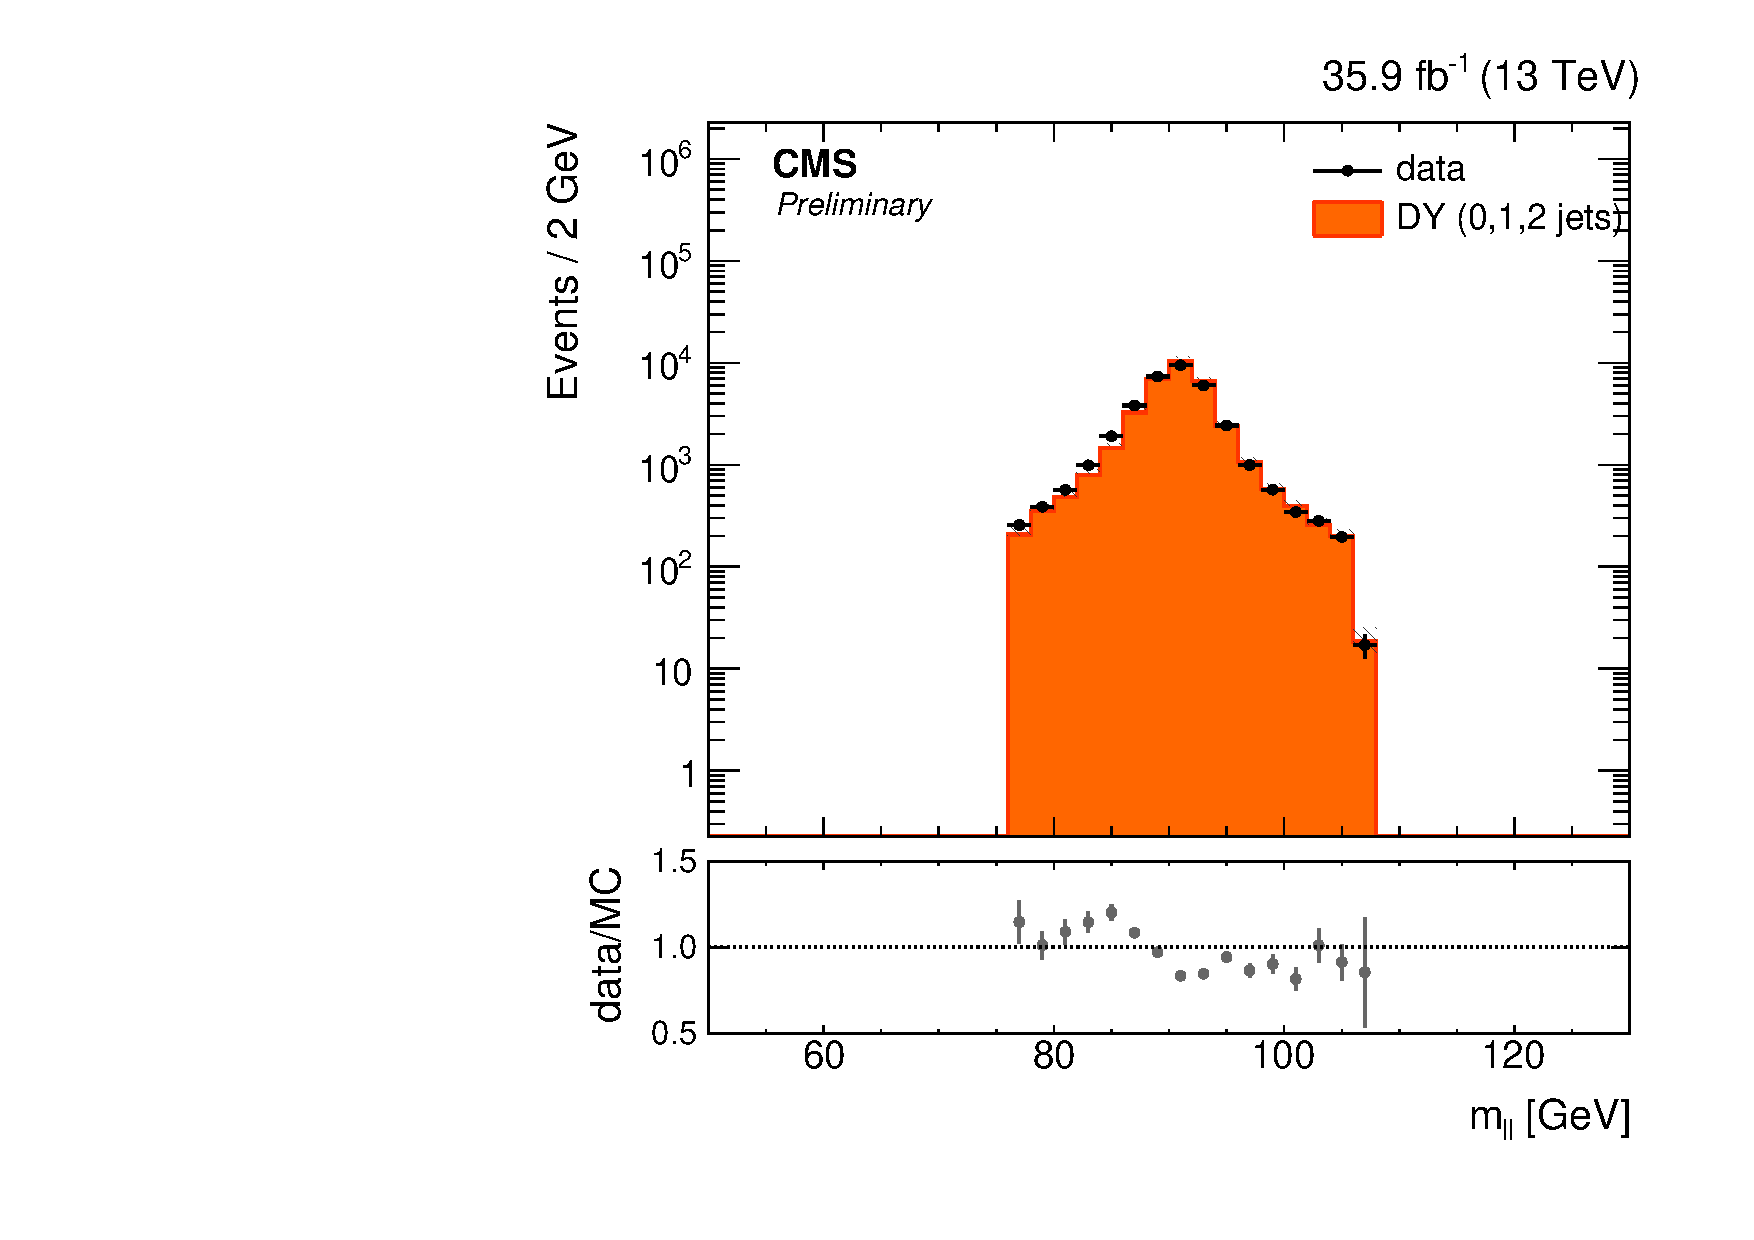
\includegraphics[width=0.4\textwidth]{figs/dilep_mass_em_bkg_sub_metbin1_ee.pdf}}
    \subfloat[$75\:\GeV<\ptmiss<100\:\GeV$]     {\label{subfig:Zpeak_metbin2_ee}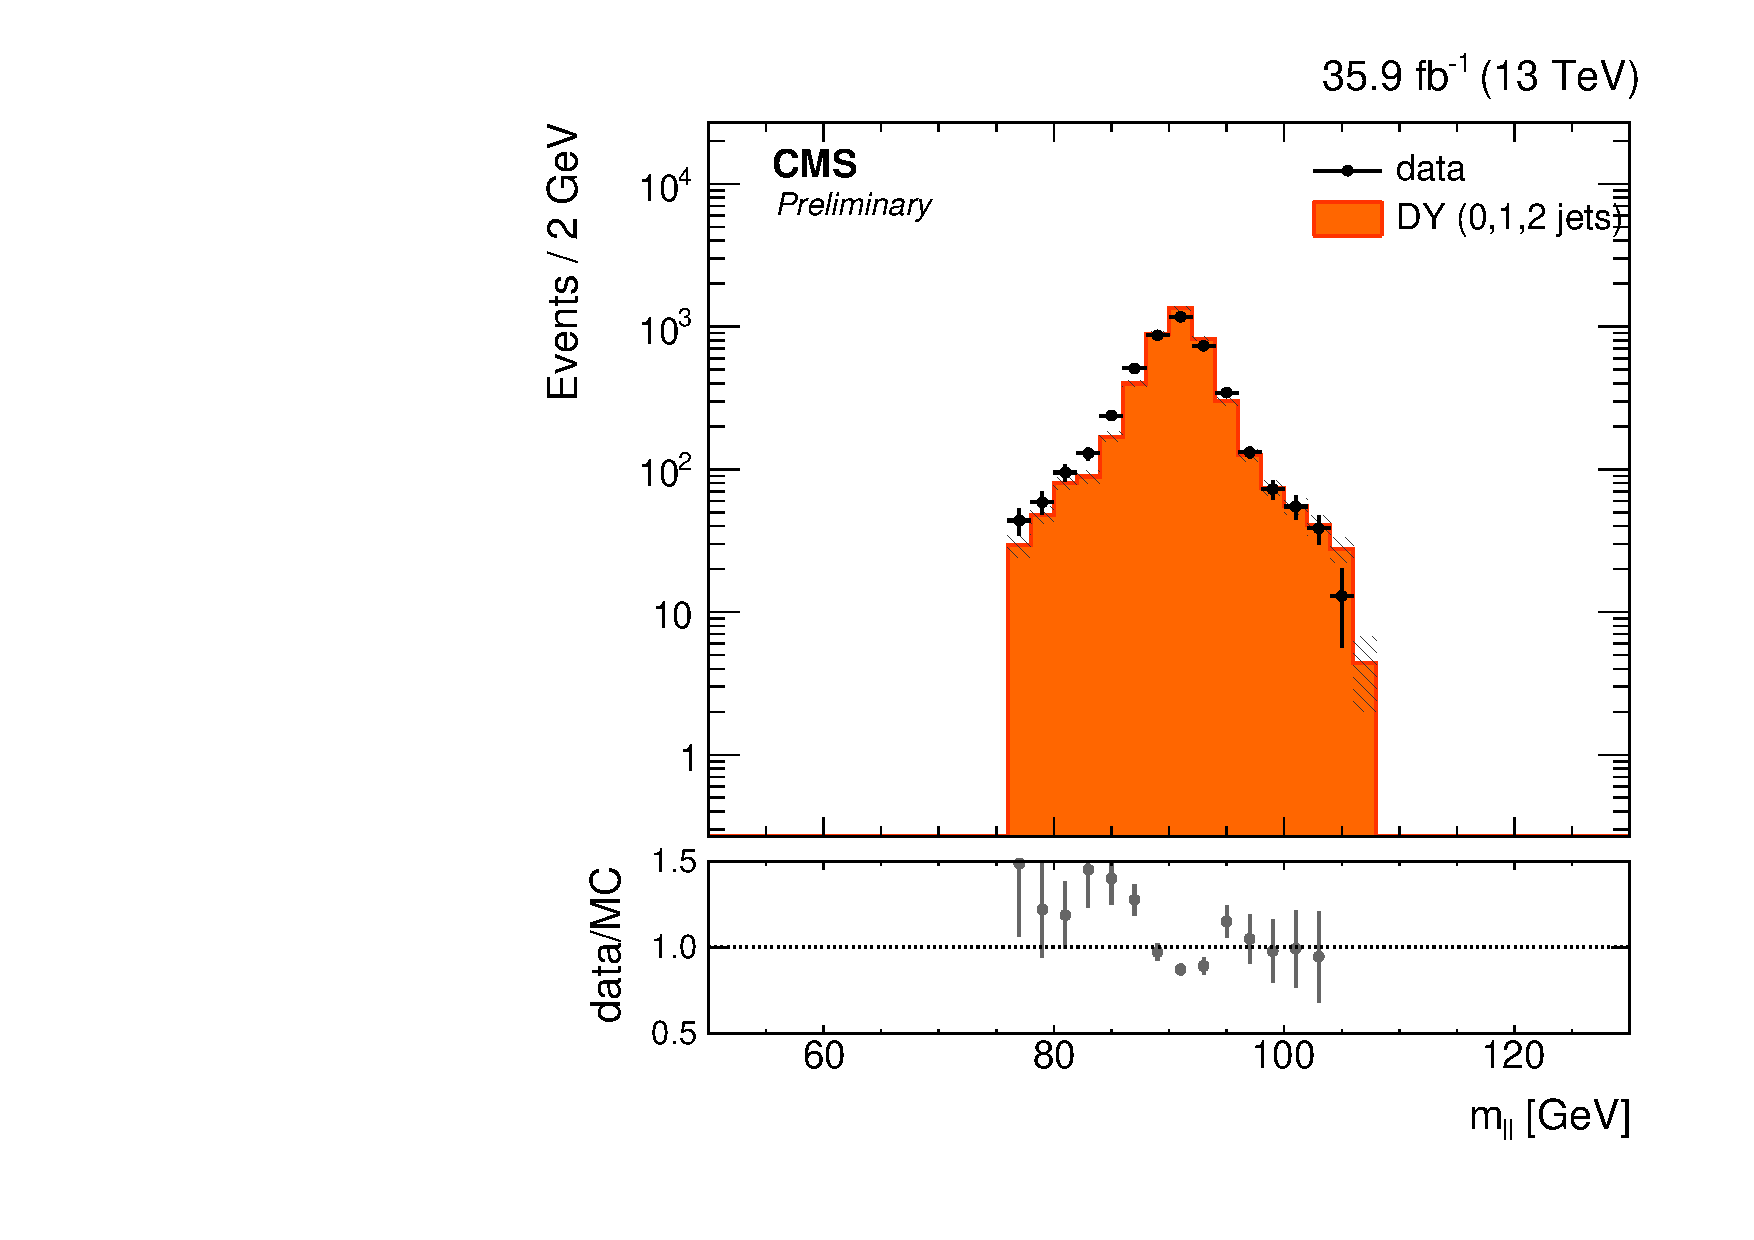
\includegraphics[width=0.4\textwidth]{figs/dilep_mass_em_bkg_sub_metbin2_ee.pdf}} \\
    \subfloat[$100\:\GeV<\ptmiss<150\:\GeV$]    {\label{subfig:Zpeak_metbin3_ee}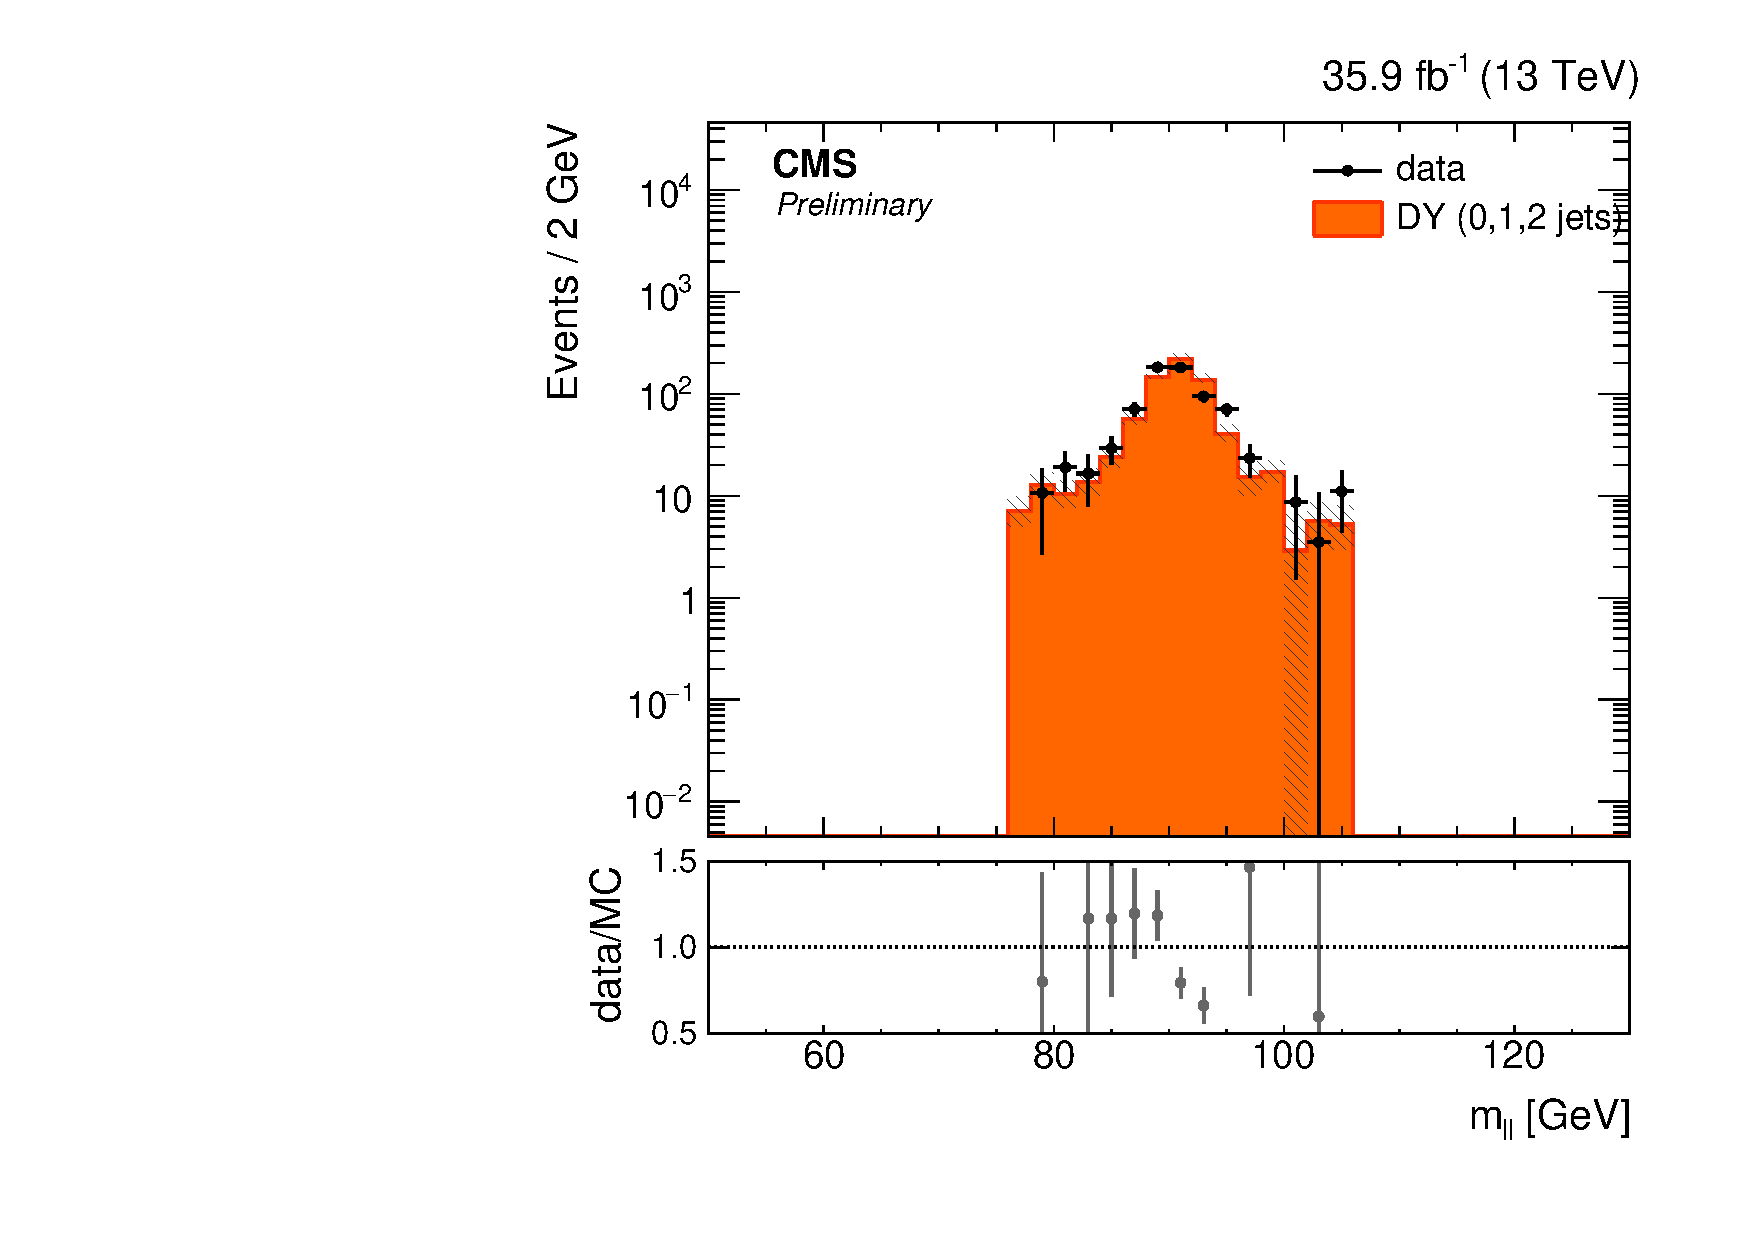
\includegraphics[width=0.4\textwidth]{figs/dilep_mass_em_bkg_sub_metbin3_ee.pdf}}
    \subfloat[$150\:\GeV<\ptmiss<1000\:\GeV$]   {\label{subfig:Zpeak_metbin4_ee}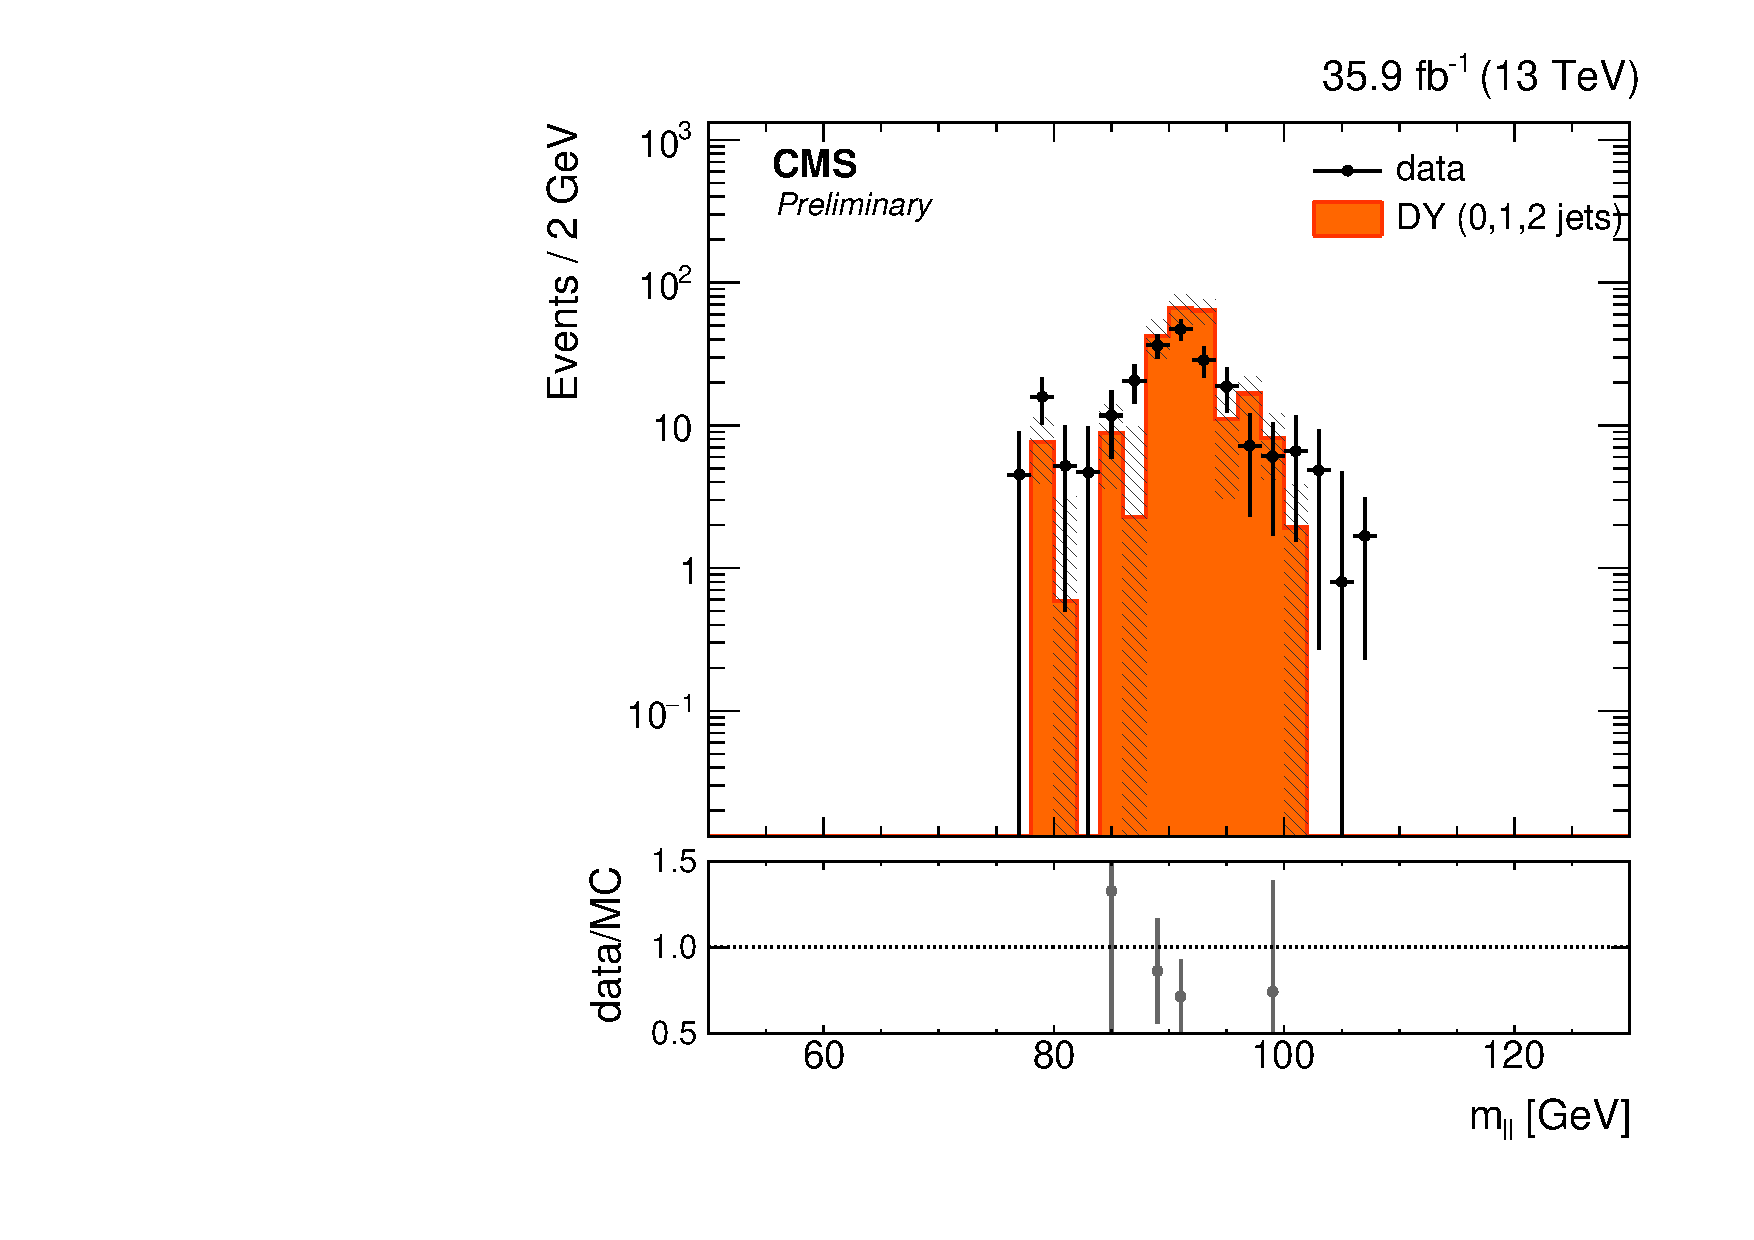
\includegraphics[width=0.4\textwidth]{figs/dilep_mass_em_bkg_sub_metbin4_ee.pdf}}
    \caption{Z peak in data and MC after subtraction of non-Drell-Yan contribution estimate from opposite-flavor data events in the $ee$ channel for various $\ptmiss$ bins.}
    \label{fig:Zpeak_ee}
  \end{center}
  \label{tab:Rinout_SF_mm}
\end{figure}

\begin{figure}
  \begin{center}
    \subfloat[$50\:\GeV<\ptmiss<75\:\GeV$]  {\label{subfig:Zpeak_metbin1_mm}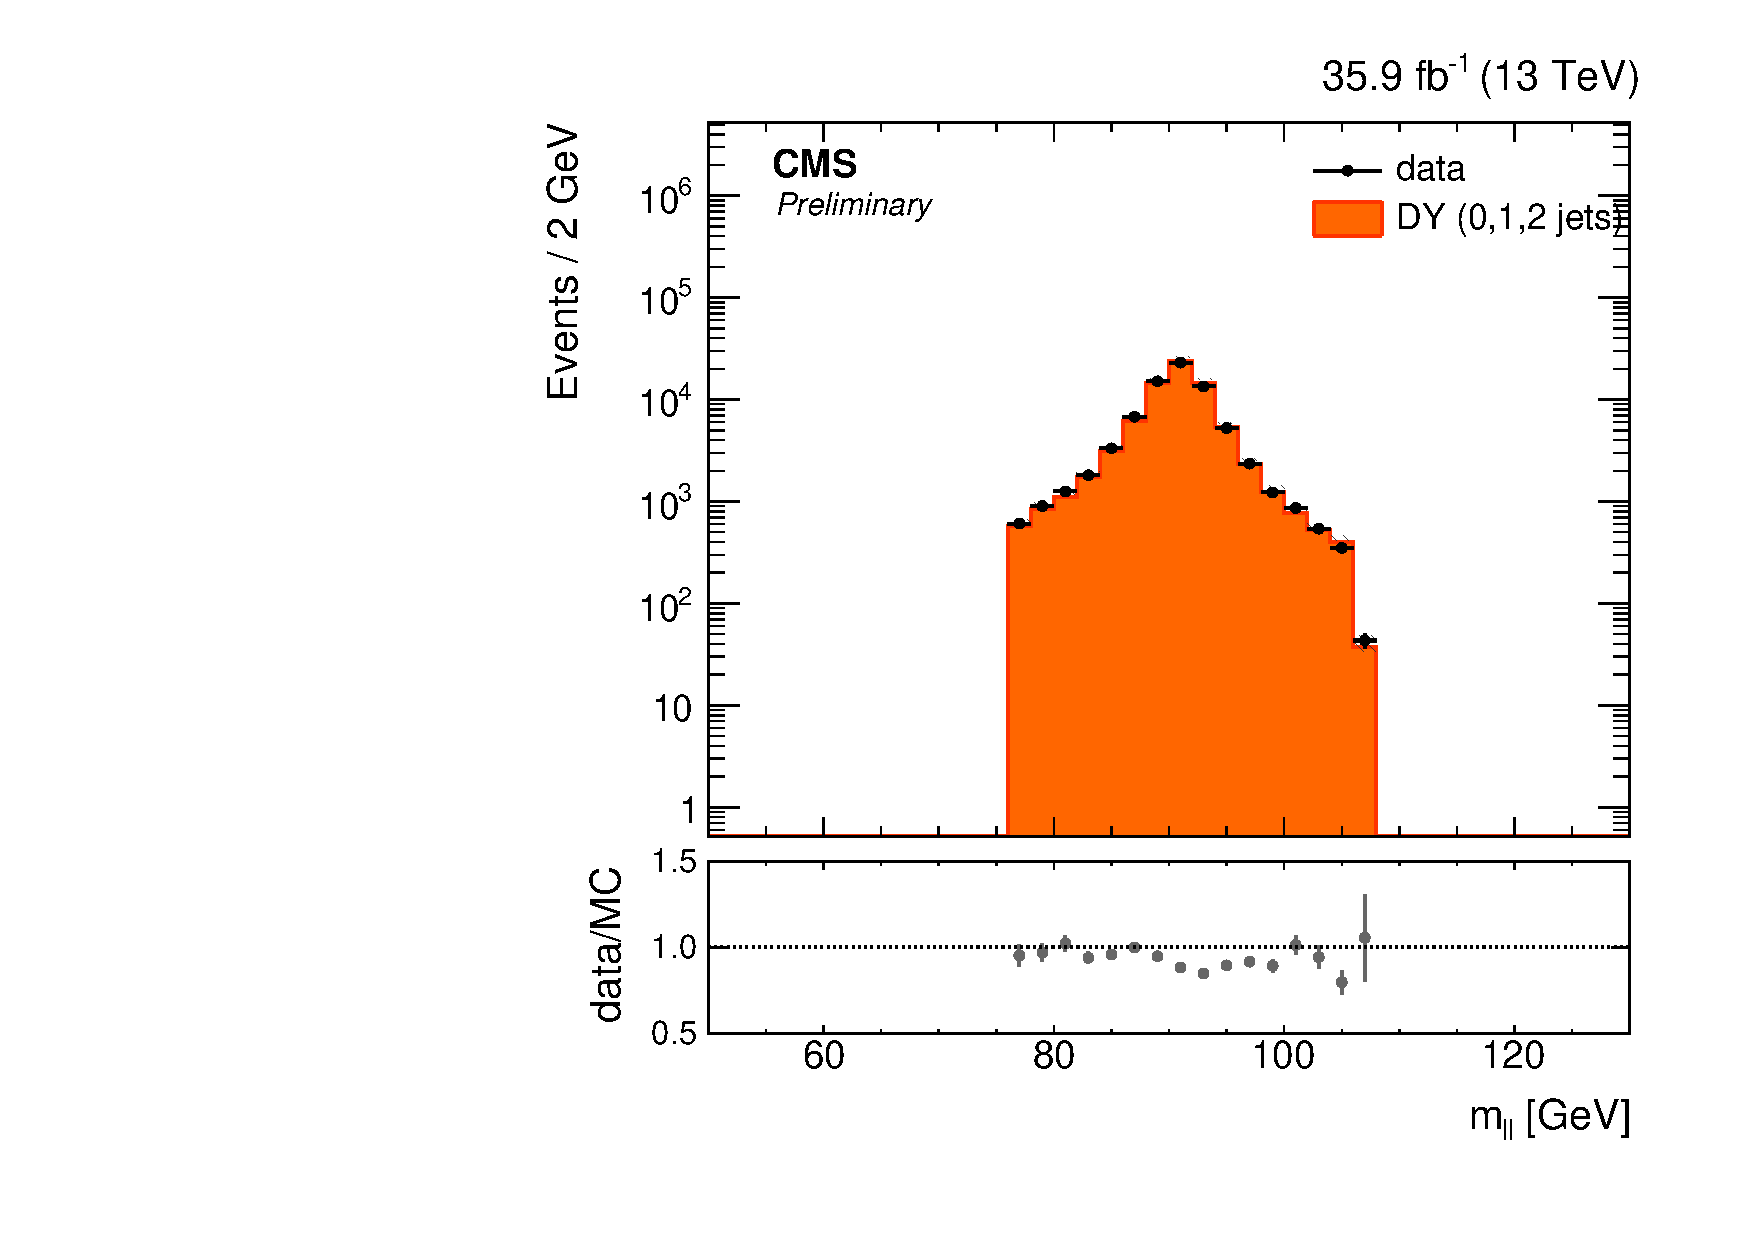
\includegraphics[width=0.4\textwidth]{figs/dilep_mass_em_bkg_sub_metbin1_mm.pdf}}
    \subfloat[$75\:\GeV<\ptmiss<100\:\GeV$] {\label{subfig:Zpeak_metbin2_mm}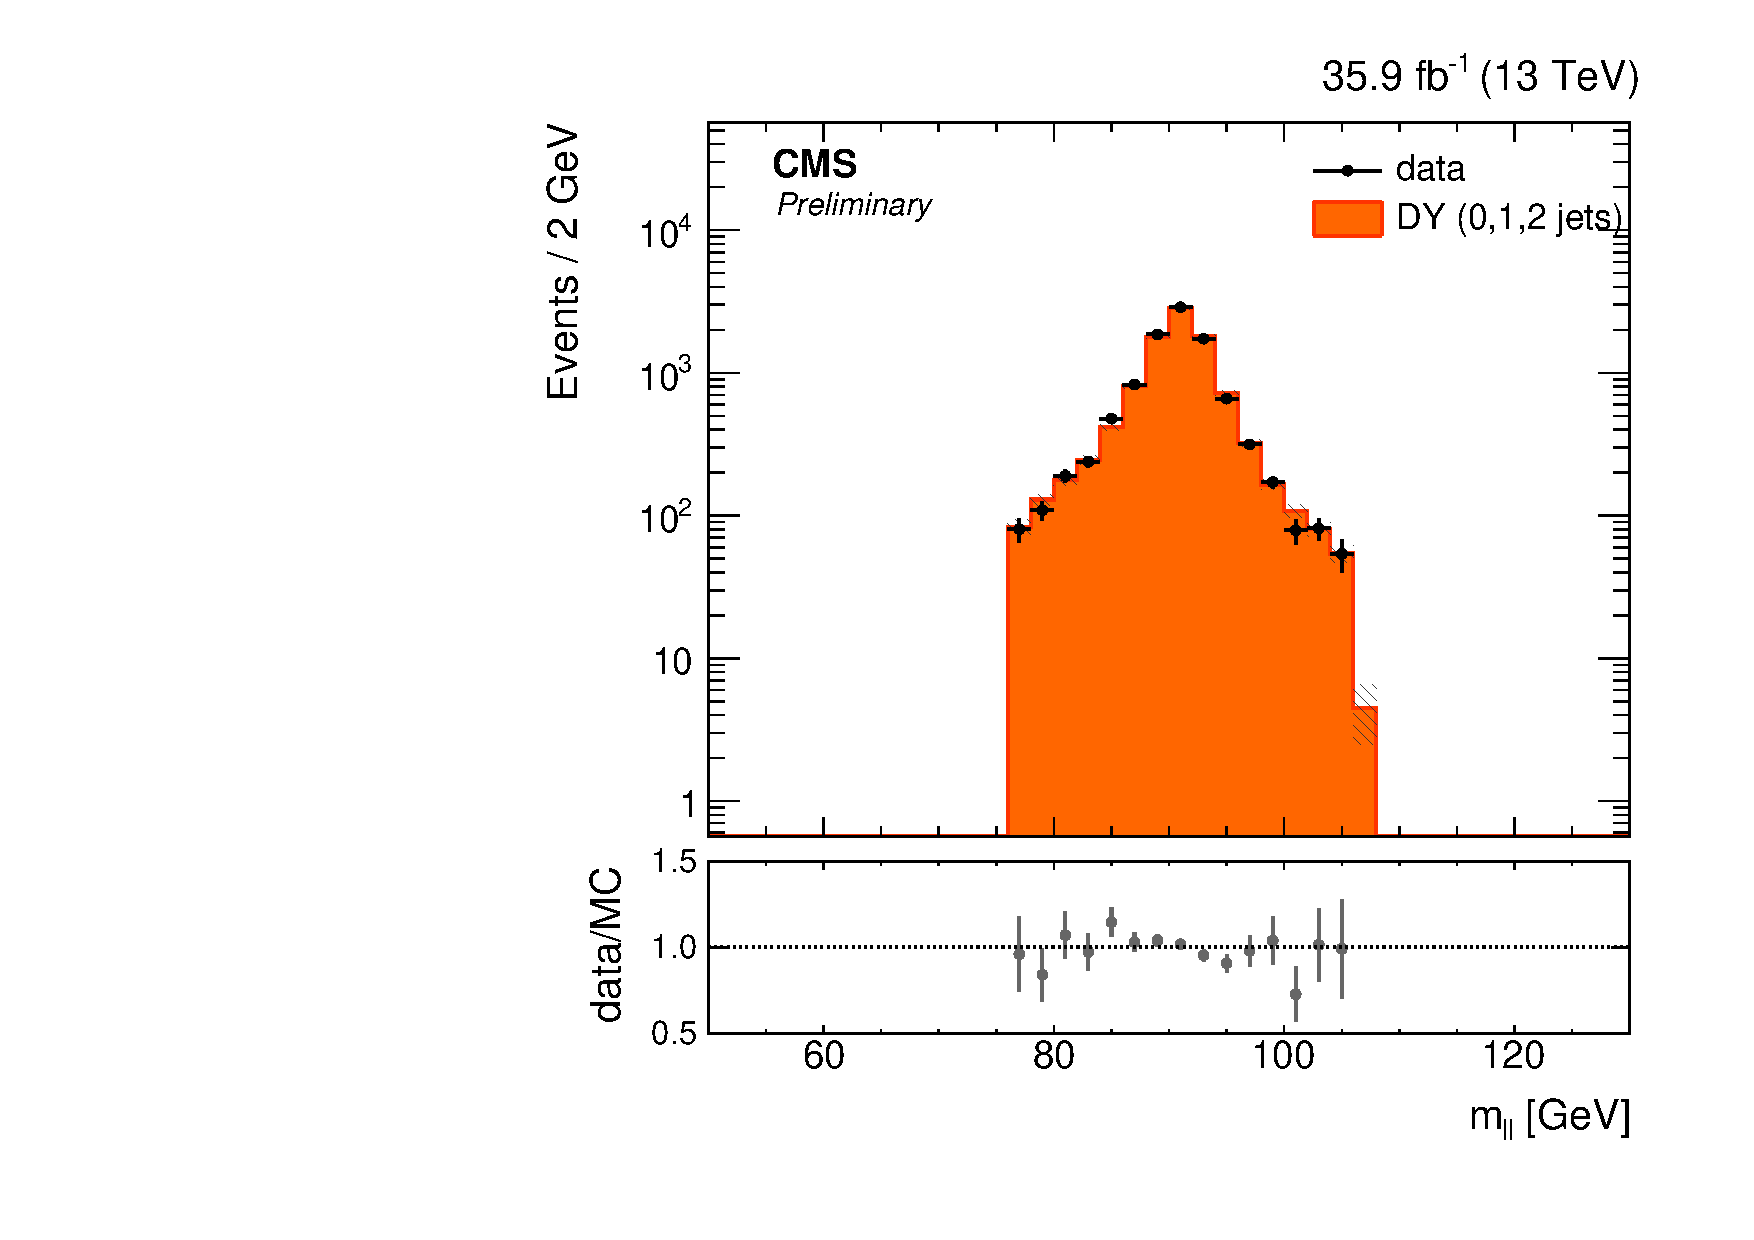
\includegraphics[width=0.4\textwidth]{figs/dilep_mass_em_bkg_sub_metbin2_mm.pdf}}\\
    \subfloat[$100\:\GeV<\ptmiss<150\:\GeV$]{\label{subfig:Zpeak_metbin3_mm}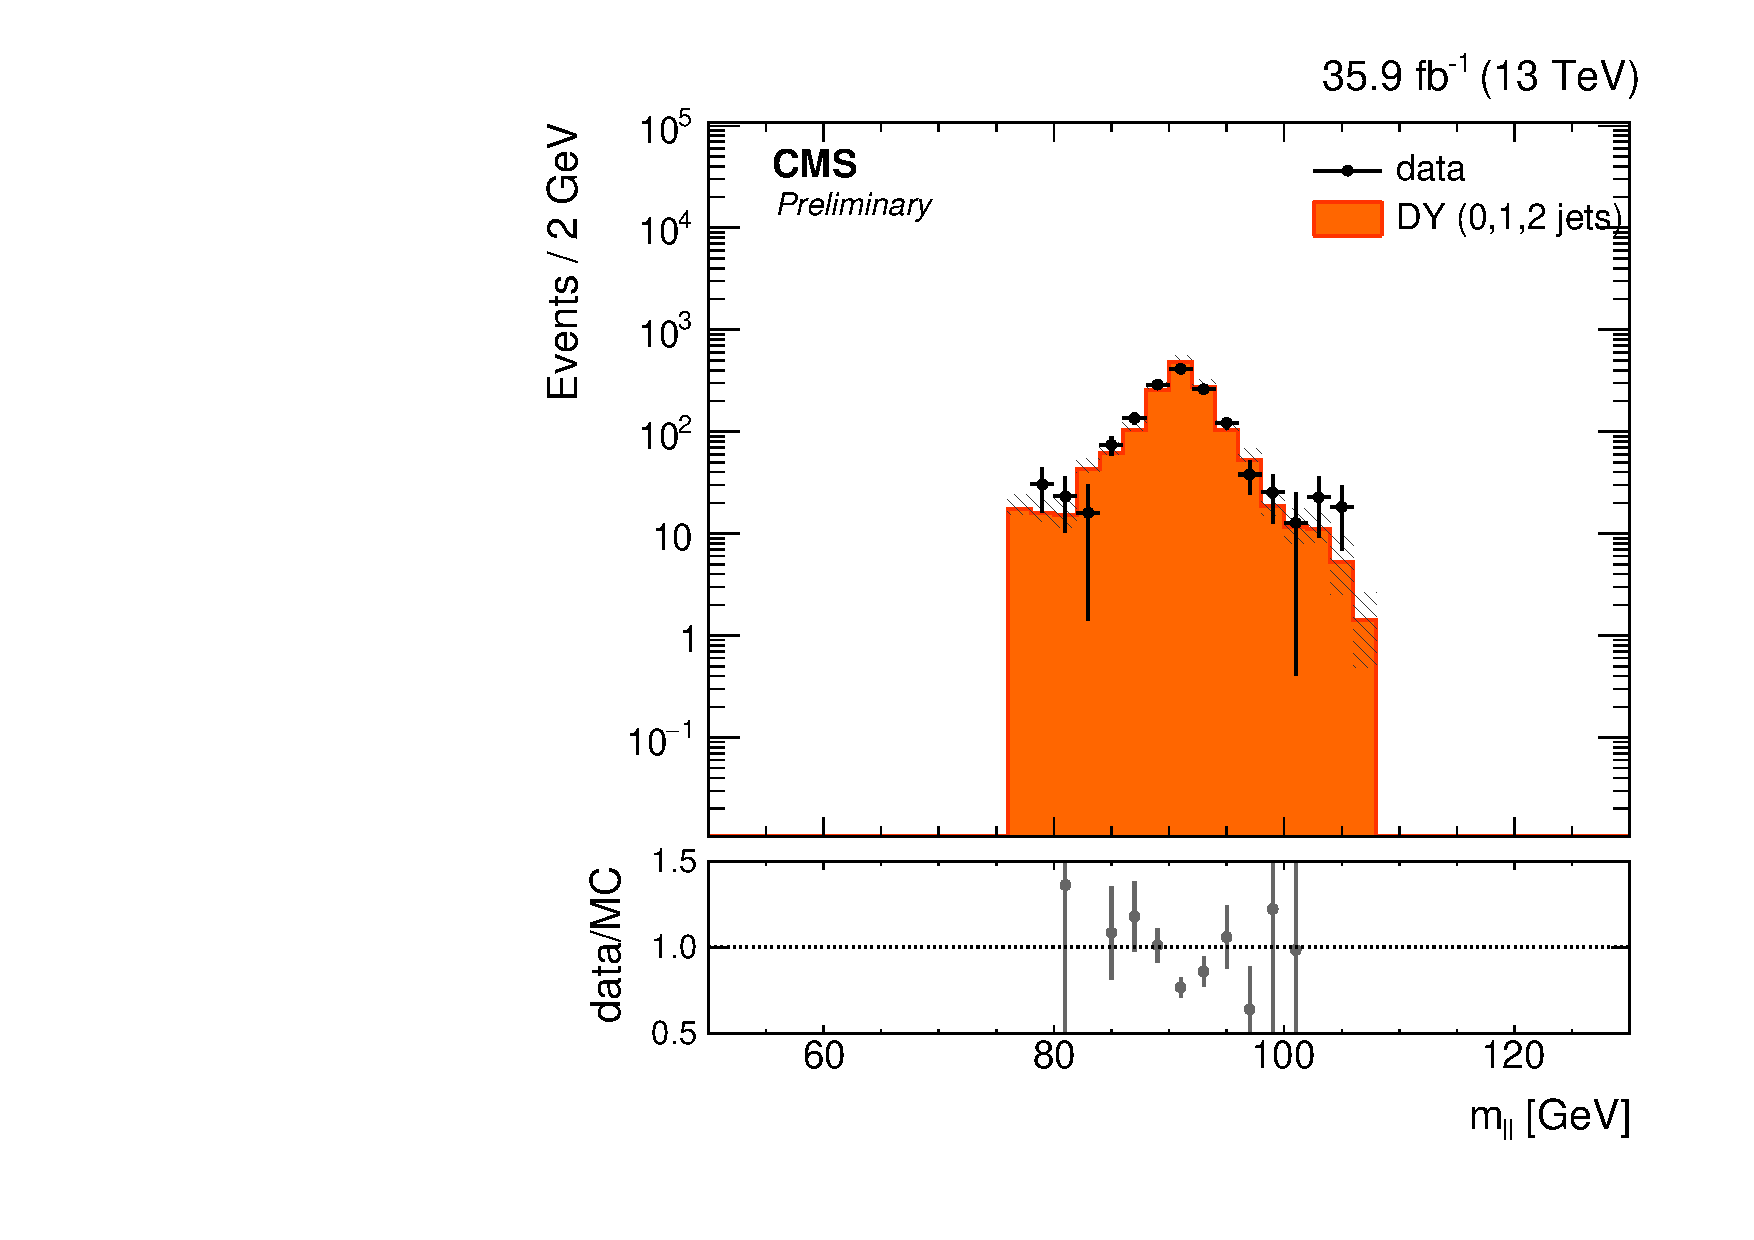
\includegraphics[width=0.4\textwidth]{figs/dilep_mass_em_bkg_sub_metbin3_mm.pdf}}
    \subfloat[$150\:\GeV<\ptmiss<1000\:\GeV$]{\label{subfig:Zpeak_metbin4_mm}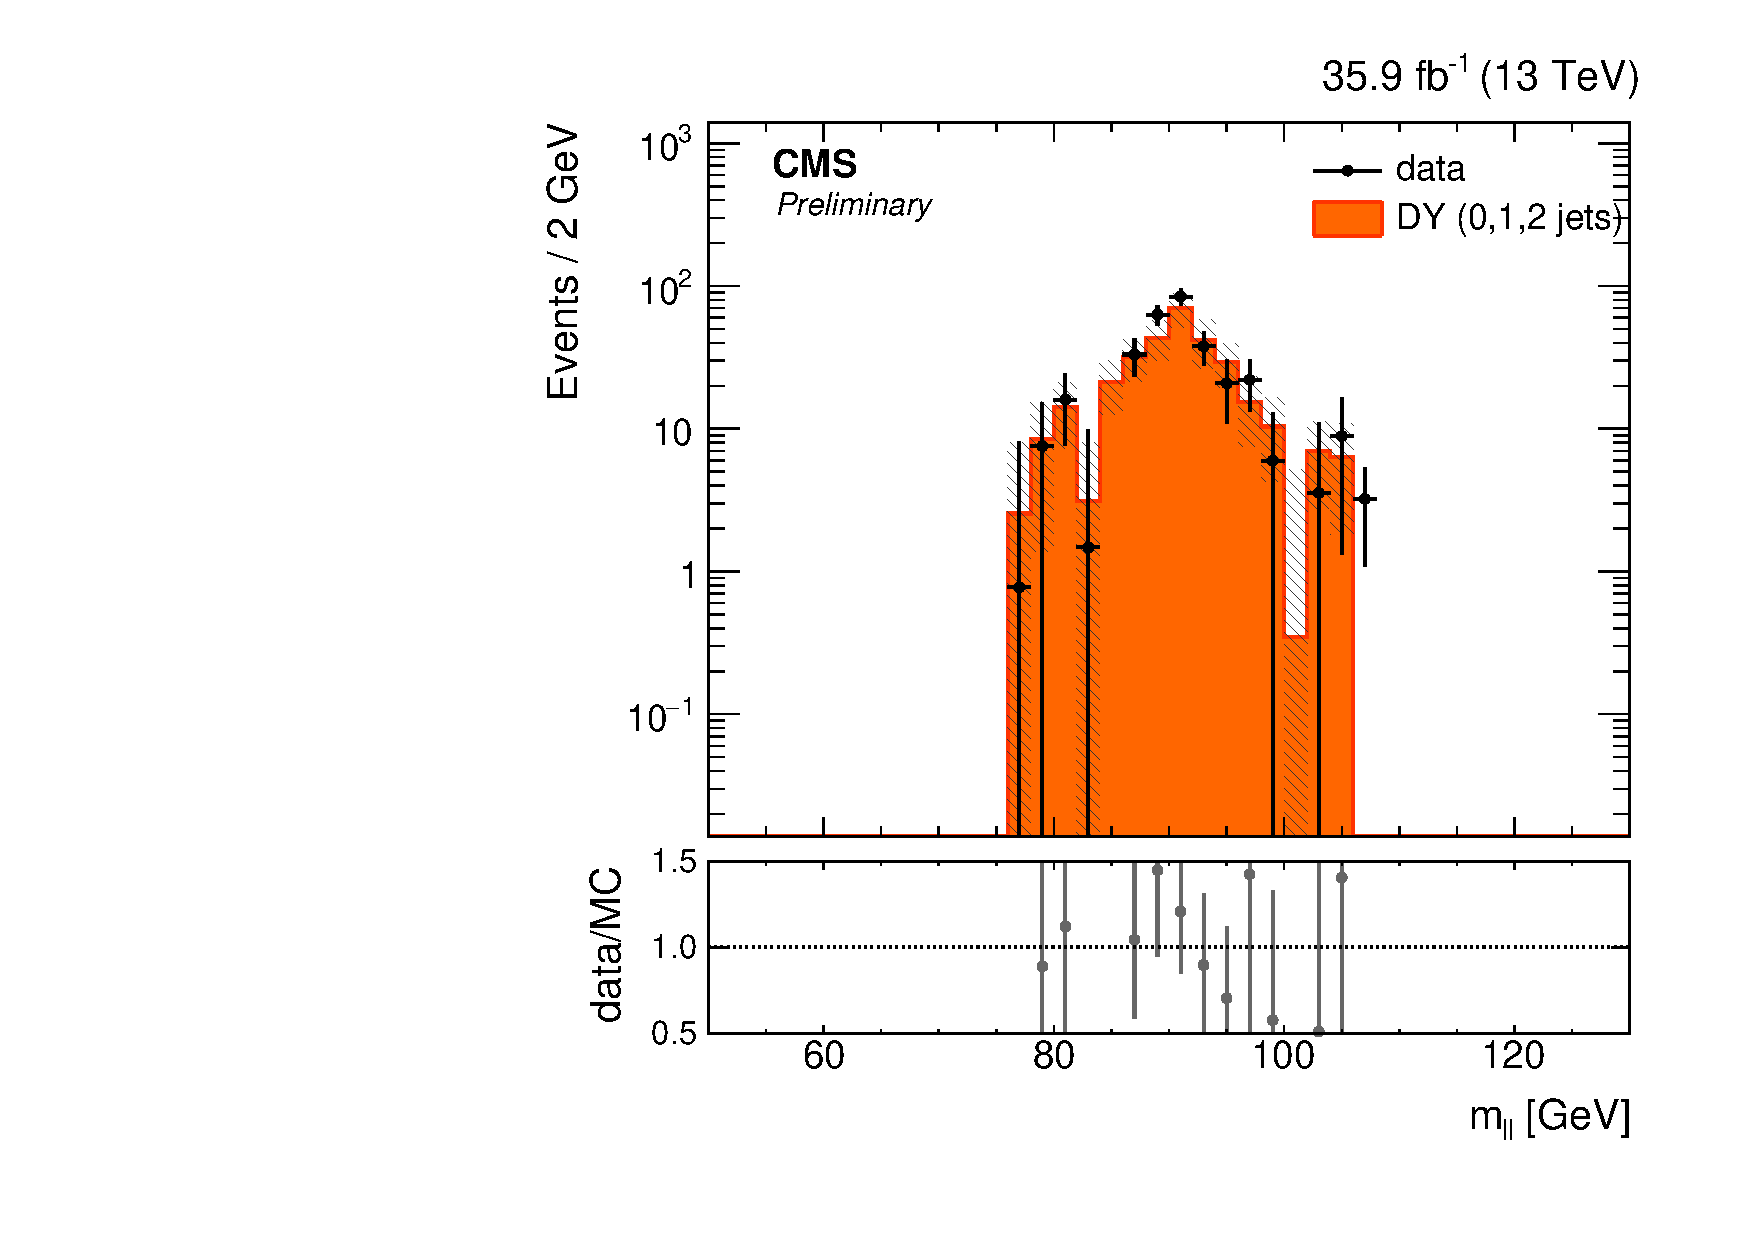
\includegraphics[width=0.4\textwidth]{figs/dilep_mass_em_bkg_sub_metbin4_mm.pdf}}
    \caption{Z peak in data and MC after subtraction of non-Drell-Yan contribution estimate from opposite-flavor data events in the $\mu\mu$ channel for various $\ptmiss$ bins.}
    \label{fig:Zpeak_mm}
  \end{center}
\end{figure}

\begin{figure}
  \centering
  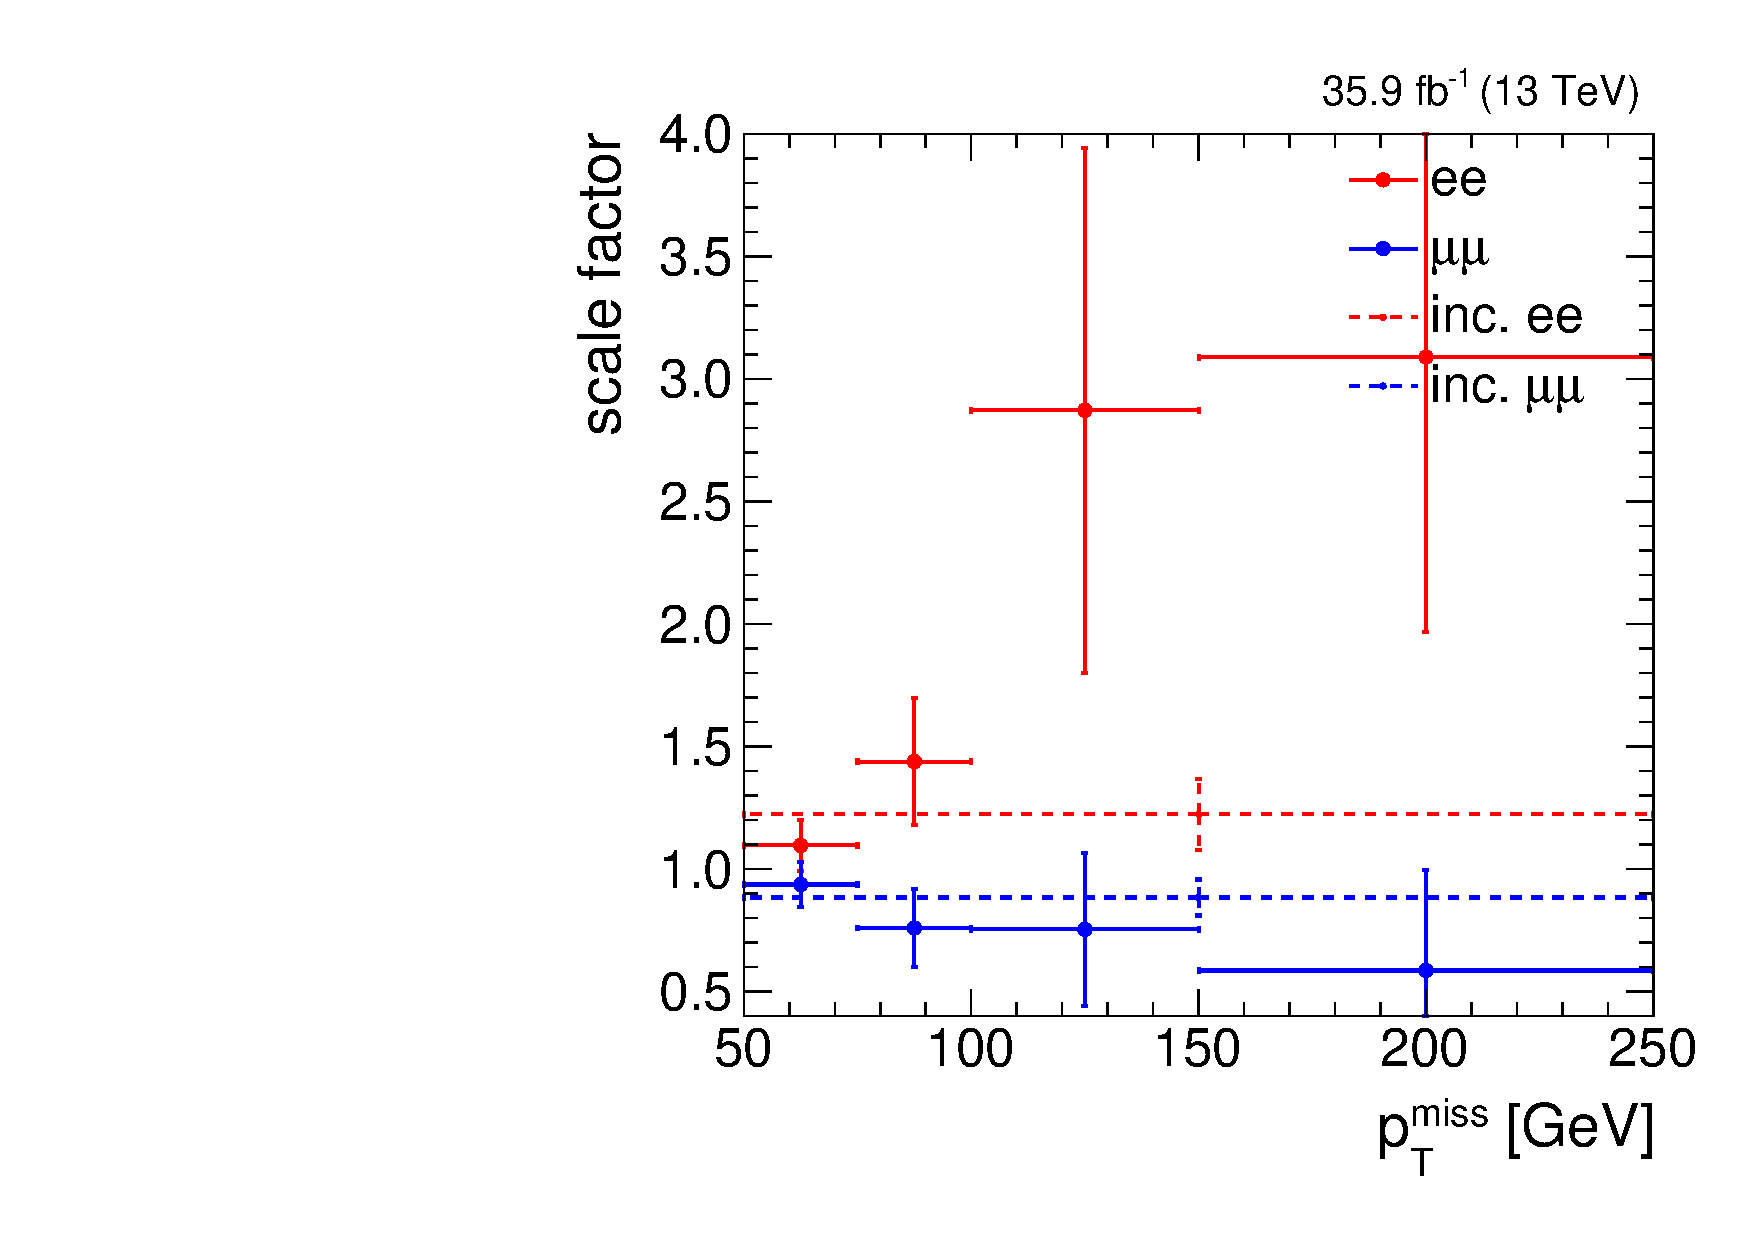
\includegraphics[width=0.48\textwidth]{figs/metbinned_Rinout_SFs.pdf}       
  \caption{Data/MC scale factors binned in $\ptmiss$ applied to MC events used for the estimate of the Drell-Yan normalization in the dilepton channel signal regions.}
  \label{fig:RinoutSFs}
\end{figure}

\clearpage

%%------------------------- Fakes -------------------------%%  
\section{Fake lepton background}
\label{sec:fakes}
\begin{figure}
  \subfloat[][\Wjets]{\label{fig:wjets}
    \feynmandiagram[vertical=b to c]{
      a [particle=\(u\)] -- [fermion] b -- [fermion] c -- [fermion] d [particle=\(\bar{d}\)],
      b -- [boson, edge label=\(W^{+}\)] f,
      e [particle=\(\ell^{+}\)] -- [fermion] f -- [fermion] g [particle=\(\nu_{\ell}\)],
      c -- [gluon, edge label=\(g\)] i,
      j [particle=\(\bar{b}\)] -- [fermion] i -- [fermion] h [particle=\(b\)],
      %        g -- [opacity=0.0001] h,
      %        a -- [opacity=0.0001] d,
      f -- [opacity=0.0001] i,
    };
  } 
  \hspace{1.0 cm}
  \subfloat[][$t\bar{t}(1\ell)$]{\label{fig:tt1l}
    \feynmandiagram[horizontal=b to c]{
      a [particle=\(g\)] -- [gluon] b -- [gluon] c,
      d [particle=\(g\)] -- [gluon] b,
      e -- [fermion, edge label=\(\bar{t}\)] c,
      g [particle=\(\bar{b}\)] -- [fermion] e,
      e -- [boson, edge label=\(W^-\)] h,
      c -- [fermion, edge label=\(t\)] f,
      e -- [opacity=0.0001] f,
      f -- [fermion] i [particle=\(b\)],
      f -- [boson, edge label'=\(W^+\)] j,
      k [particle=\(\bar{\nu}_{\ell}\)] -- [fermion] h -- [fermion] l [particle=\(\ell^-\)],
      m [particle=\(\bar{q}\)] -- [fermion] j -- [fermion] n [particle=\(q\)],
    };
  }
  \caption{Examples of~\protect\subref{fig:wjets} \Wjets, and ~\protect\subref{fig:tt1l} semileptonic \ttbar that contribute to the fake lepton background.}
  \label{fig:fakes_feyn}
\end{figure}


Another type of reducible background, the fake (or non-prompt) lepton background, is also estimated using observed events. Processes which are expected to contain only one prompt electron or muon in the final state may pass the signal region selection as described in Sec.~\ref{sec:selection} by a jet-induced faking of a second lepton. Namely, processes such as \Wjets, semileptonic decays of \ttbar and tW associated production, and leptonic single top decays, a few of which are shown in~\FigureRef{fig:fakes_feyn}, comprise the fake lepton background processes. 

The data-driven technique used to estimate the relative contribution of fake lepton backgrounds in the signal regions is based on the measurement of the fake rate. This rate is obtained from a sample in data which is enriched in QCD multijet events. Very loose working points for an electron object and muon object are define; these are called ``fake-able objects'' (``FO'') and their definitions are found under the heading ``FO WP'' in Tables~\ref{tab:ele_wp} and~\ref{tab:muon_wp} for electrons and muons respectively.

The method has two main steps,
\begin{enumerate}
\item \textbf{Measurement:} in a QCD enriched sample in data, measure the probability of a ``FO'' to pass ``Tight'' lepton selection: the ``fake rate''
\item \textbf{Application:} in a sample consisting of one ``Tight'' lepton and one ``FO'' that fails ``Tight'' selection, use the fake rate to estimate the background in the signal region
\end{enumerate}

\subsection{Fake rate measurement}
\label{subsec:fr_measure}
To obtain a sample enriched in jet-induced fakes in order to perform the fake rate measurement, the following selection is applied,
\begin{itemize}
\item Event passes one of the following triggers:
  \begin{itemize}
  \item HLT\_Ele$[12, 23]$\_CaloIdM\_TrackIdM\_PFJet30
  \item HLT\_Ele$[12, 23]$\_CaloIdL\_TrackIdL\_IsoVL\_PFJet30
  \item HLT\_Mu$[8, 17]$\_TrkIsoVVL
  \end{itemize}
\item there is exactly one ``FO'' in the event, matched to the trigger that fired
\item \ptmiss<40\:\GeV
\item $M_{T}<35\:\GeV$
\item at least one jet with $\pt>30\:\GeV$ and $|\eta|<4$
\item $\Delta\phi>2$ between the leading jet in the event and the ``FO''
\end{itemize}
The cuts are chosen to suppress the \Wjets contribution (i.e. the low $M_{T}$ requirement), and to enhance the multi-jet QCD contribution. Even then, the level of contamination from electroweak processes (\Wjets, \Zjets, \ttbar) in this sample ranges from $10\%$ at low \pt to $70\%$ at high \pt. The contamination is thus significant, particularly in the measurement sample for muon ``FO'', that a subtraction of prompt, real leptons must be done (based on expectations from simulation). The fake rate (FR) is defined as the efficiency of a ``FO'' to pass ``Tight'' requirements,
\begin{equation}
  \text{FR}_{ij} = \Big[\frac{\left(N^{\text{data}}_{Tight} - N^{\text{EWK}}_{Tight}\right)}{\left(N^{\text{data}}_{FO} - N^{\text{EWK}}_{FO}\right)}\Big]_{i=\eta\,j=\pt}
\end{equation}
The measured fake rates are listed in Tables~\ref{tab:ele_fr} and~\ref{tab:muon_fr}. The fake rates depend more strongly on \eta than on \pt as shown in Fig.~\ref{fig:ele_fr_plots} and Fig.~\ref{fig:muon_fr_plots}.

\begin{table}[!ht]
\centering
\scalebox{0.9}
{
\begin{tabular}{|c|c|c|c|c|c|}
\hline
                & $0.0 < |\eta| < 0.5$ & $0.5 < |\eta| < 1.0$ & $1.0 < |\eta| < 1.5$ & $1.5 < |\eta| < 2
.0$ & $2.0 < |\eta| < 2.5$ \\
\hline
$10 < \pt < 15$ &  $0.063 \pm  0.008$  & $ 0.088 \pm  0.009$  &  $0.121 \pm  0.008$  &  $0.181 \pm  0.00
9$  &  $0.176 \pm  0.012$ \\
\hline  
$15 < \pt < 20$ &  $0.085 \pm  0.003$  & $ 0.085 \pm  0.003$  &  $0.106 \pm  0.003$  &  $0.164 \pm  0.00
4$  &  $0.153 \pm  0.005$ \\
\hline
$20 < \pt < 25$ & $ 0.062 \pm  0.008$  &  $0.059 \pm  0.007$  &  $0.080 \pm  0.009$  &  $0.131 \pm  0.010$  &  $0.148 \pm  0.012$ \\
\hline 
$25 < \pt < 30$ &  $0.073 \pm  0.011$  &  $0.078 \pm  0.078$  &  $0.090 \pm  0.011$  &  $0.140 \pm  0.012$  &  $0.162 \pm  0.012$ \\
\hline
$\pt > 30$      &  $0.065 \pm  0.007$  &  $0.091 \pm  0.008$  &  $0.089 \pm  0.007$  &  $0.169 \pm  0.008$  &  $0.190 \pm  0.008$ \\
\hline    
\end{tabular}   
}
\caption{Electron fake rates}
\label{tab:ele_fr}
\end{table}

\begin{table}[!ht]
\centering
\scalebox{0.9}
{
\begin{tabular}{|c|c|c|c|c|c|}
\hline
                & $0.0 < |\eta| < 0.5$ & $0.5 < |\eta| < 1.0$ & $1.0 < |\eta| < 1.5$ & $1.5 < |\eta| < 2.0$ & $2.0 < |\eta| < 2.4$ \\
\hline
$10 < \pt < 15$ &  $0.192 \pm  0.004$  & $ 0.210 \pm  0.004$  &  $0.235 \pm  0.004$  &  $0.283 \pm  0.004$  &  $0.294 \pm  0.005$ \\
\hline
$15 < \pt < 20$ &  $0.202 \pm  0.001$  & $ 0.214 \pm  0.001$  &  $0.253 \pm  0.001$  &  $0.293 \pm  0.001$  &  $0.307 \pm  0.002$ \\
\hline
$20 < \pt < 25$ & $ 0.187 \pm  0.001$  &  $0.200 \pm  0.001$  &  $0.240 \pm  0.001$  &  $0.286 \pm  0.001$  &  $0.307 \pm  0.002$ \\
\hline 
$25 < \pt < 30$ &  $0.177 \pm  0.002$  &  $0.196 \pm  0.002$  &  $0.239 \pm  0.002$  &  $0.279 \pm  0.002$  &  $0.310 \pm  0.003$ \\
\hline
$\pt > 30$      &  $0.172 \pm  0.002$  &  $0.200 \pm  0.002$  &  $0.233 \pm  0.002$  &  $0.279 \pm  0.002$  &  $0.311 \pm  0.003$ \\
\hline    
\end{tabular}   
}
\caption{Muon fake rates}
\label{tab:muon_fr}
\end{table}

\begin{figure}[htbp!]
\begin{center}
  \subfloat[][fake rates vs. \pt]    {\label{subfig:fr_vs_pt_e}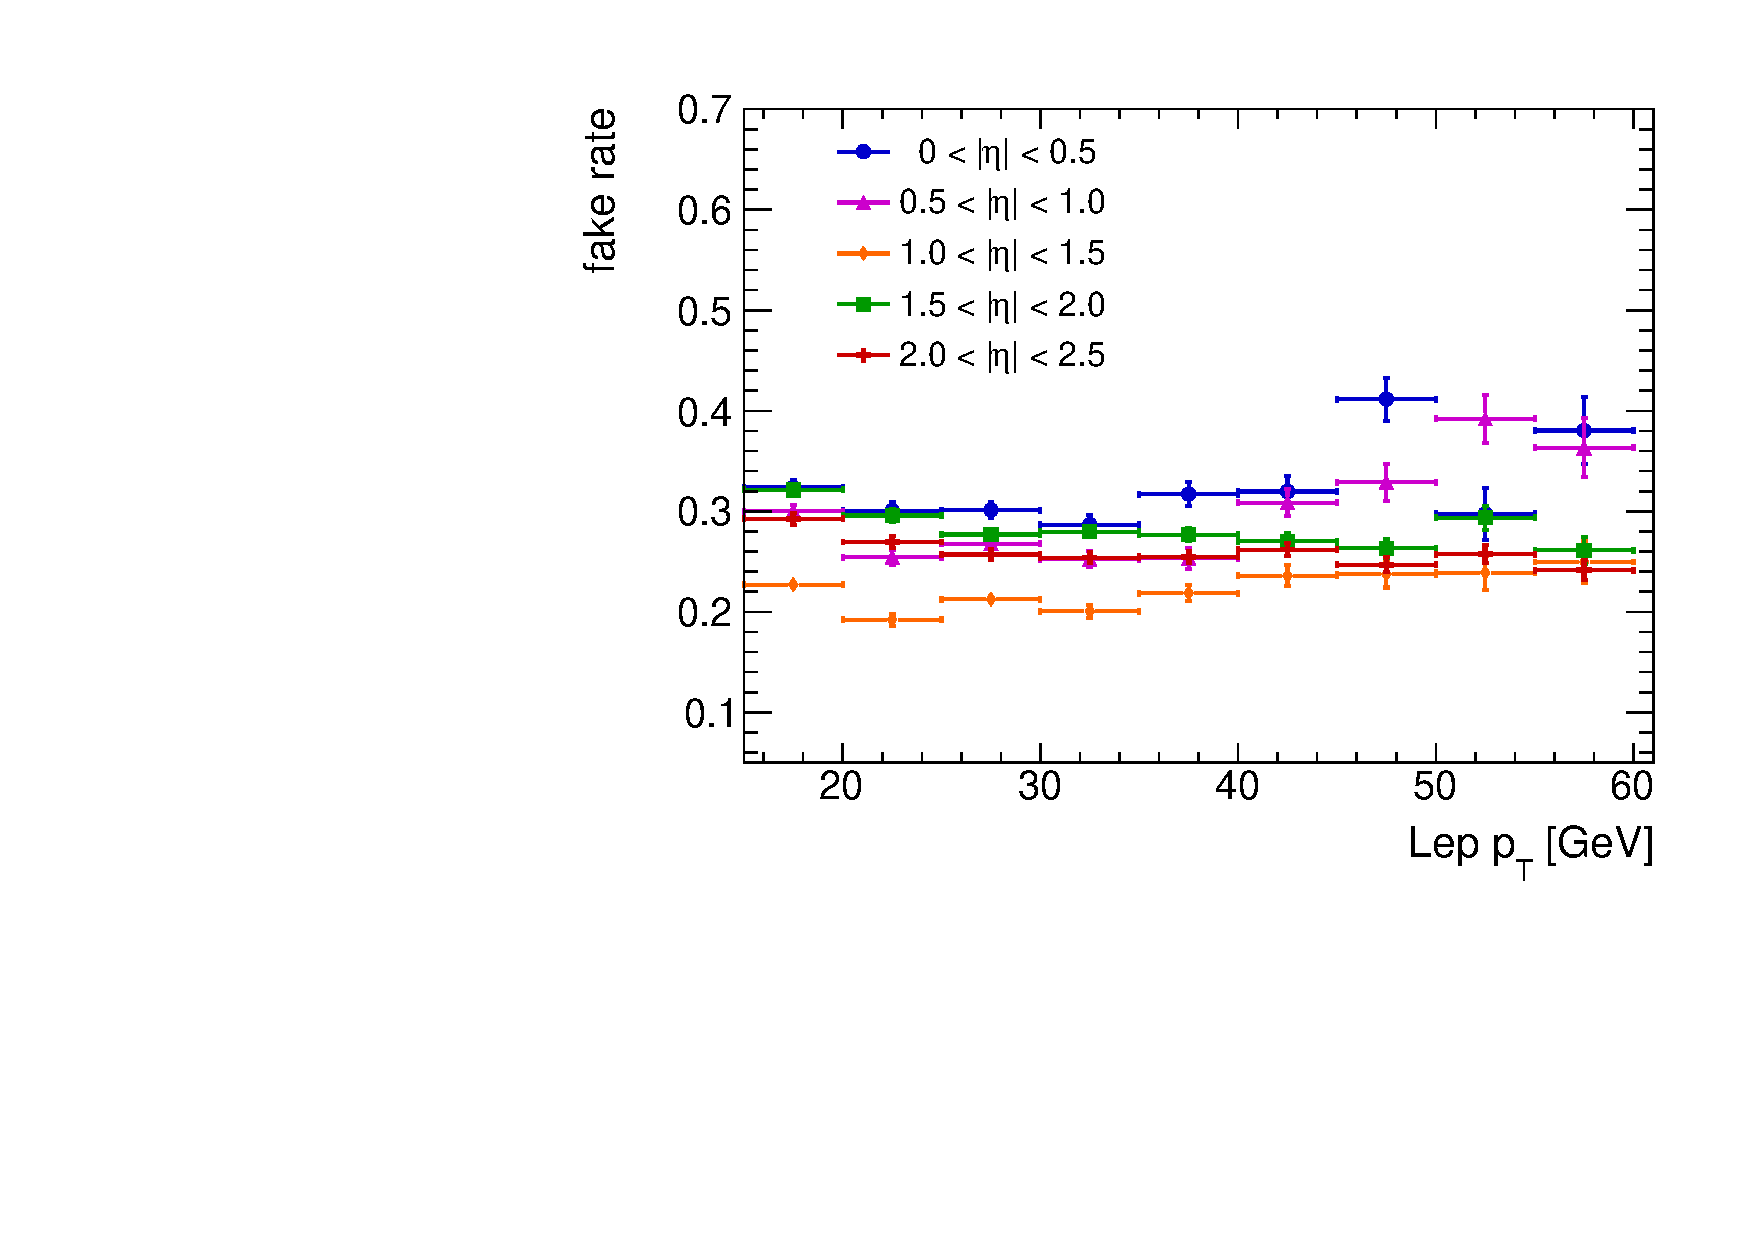
\includegraphics[width=0.45\textwidth]{figs/fakerate_v_pt_e.pdf}}
  \subfloat[][fake rates vs. $|\eta|$]  {\label{subfig:fr_vs_eta_e}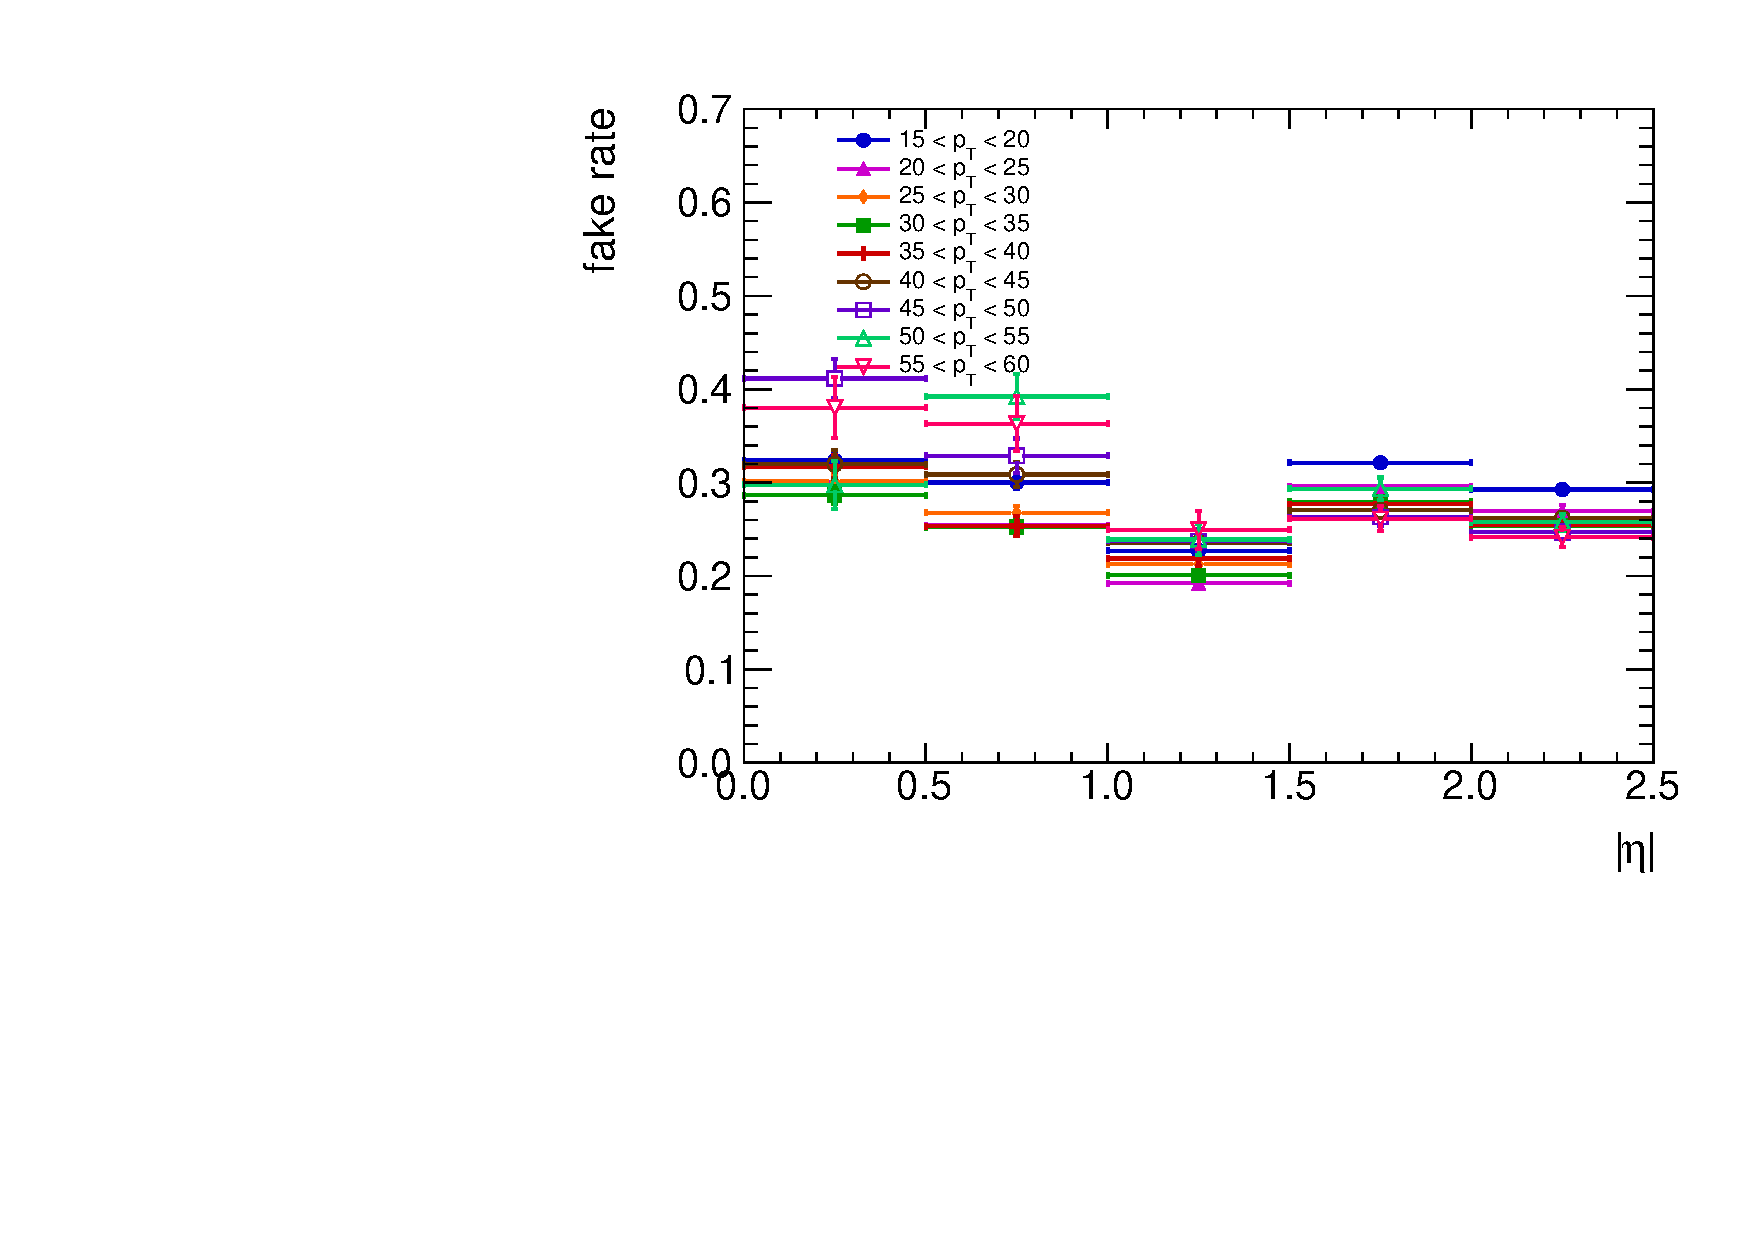
\includegraphics[width=0.45\textwidth]{figs/fakerate_v_eta_e.pdf}}
  \caption{Measured electron fake rates as a function of lepton ~\protect\subref{subfig:fr_vs_pt_e} $\pt$ and ~\protect\subref{subfig:fr_vs_eta_e} $|\eta|$.}
  \label{fig:ele_fr_plots}
\end{center}
\end{figure}

\begin{figure}[htbp!]
\begin{center}
  \subfloat[][fake rates vs. \pt]    {\label{subfig:fr_vs_pt_m}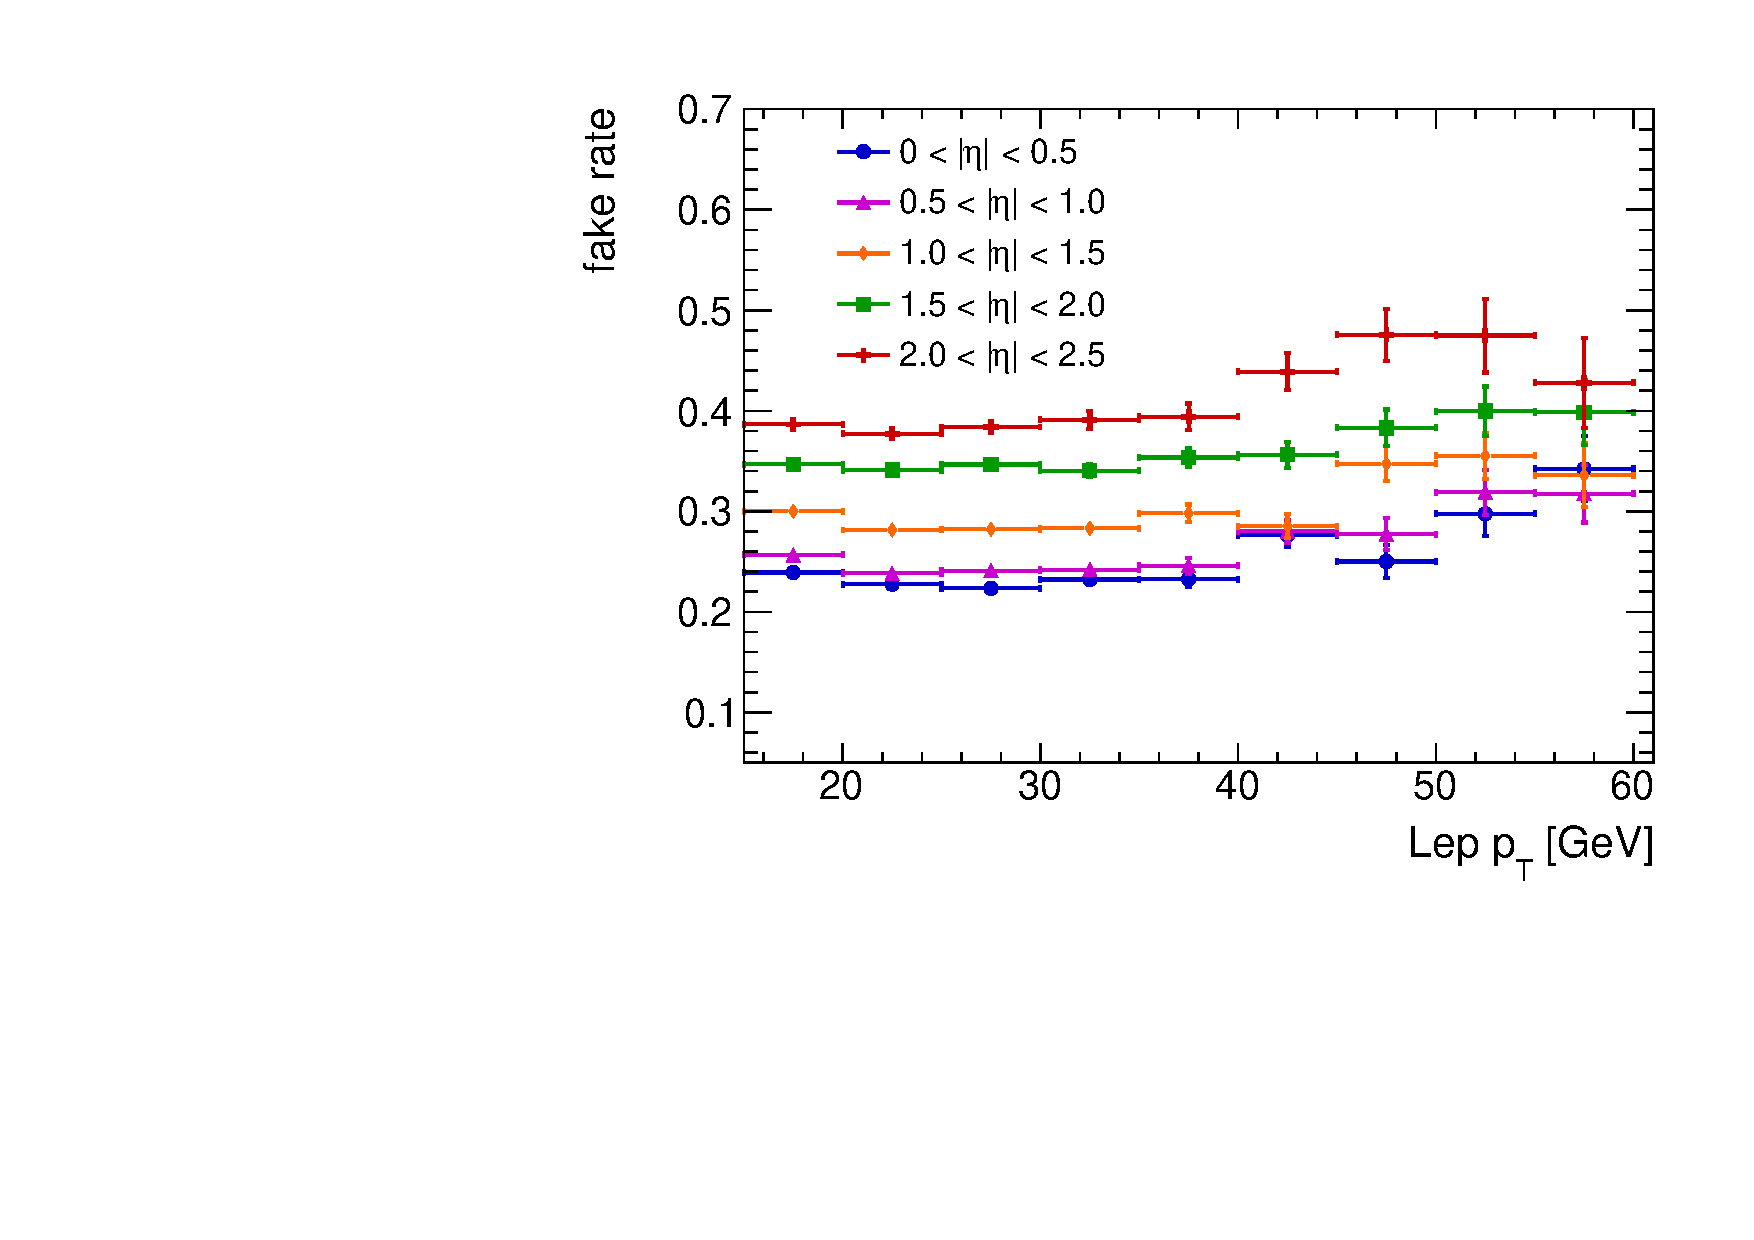
\includegraphics[width=0.45\textwidth]{figs/fakerate_v_pt_m.pdf}}
  \subfloat[][fake rates vs. $|\eta|$]  {\label{subfig:fr_vs_eta_m}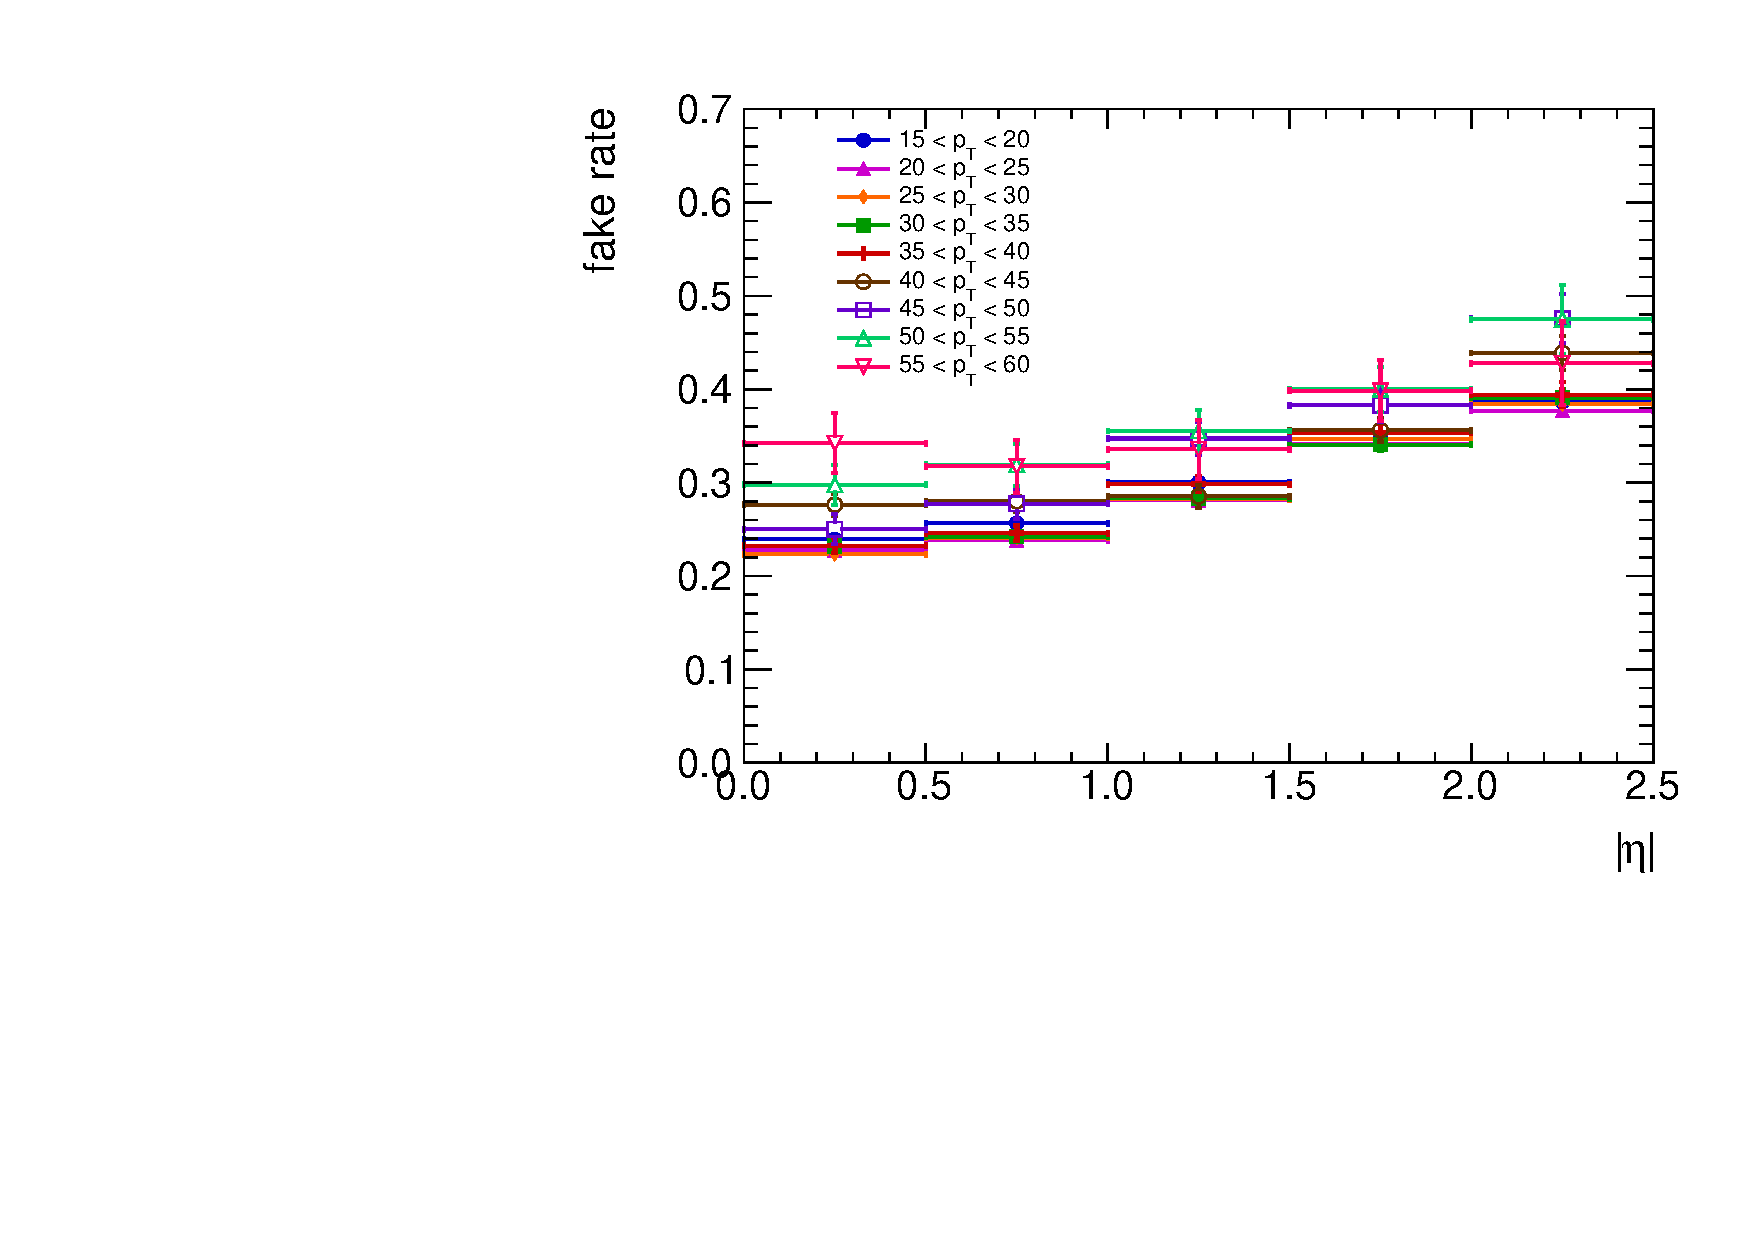
\includegraphics[width=0.45\textwidth]{figs/fakerate_v_eta_m.pdf}}
  \caption{Measured muon fake rates as a function of lepton ~\protect\subref{subfig:fr_vs_pt_e} $\pt$ and ~\protect\subref{subfig:fr_vs_eta_e} $|\eta|$.}
  \label{fig:muon_fr_plots}
\end{center}
\end{figure}

\subsection{Fake rate application}
\label{subsec:fr_app}
The FR does not give a direct measure for an absolute lepton fake rate; it is the probability for a fake lepton which passes loose identification criteria, to additionally pass tight identification and isolation criteria. Thus, to perform the estimate of the fake lepton background, an application sample of ``Tight''$+$``FO'' pairs are obtained by requiring the signal selection with the only modification being that instead of two ``Tight'' leptons, one ``Tight'' lepton and one ``FO'' that fails ``Tight'' selection is required. Each pair is then assigned a weight, FR/$(1-\mbox{FR})$, corresponding to a likelihood that the ``FO'' in the pair will be promoted to a ``Tight'' lepton, and the sum of these weighted pairs give a prediction for the background yield and distributions. In principle, a single event can contribute multiple ``Tight''$+$``FO'' pairs to the application sample, but in practice there is rarely more than one pair from an event.

Dileptonic processes can contaminate the application sample and needs to be subtracted off. MC expectations are used to perform the subtraction; about $95\%$ of this contamination comes from dileptonic $\ttbar$ events.

\subsection{Fake rate closure test}
\label{subsec:fr_close}
As a way to validate the estimation procedure, a closure test is performed in a fakes enriched region. The events in this region are required to pass the same selection as for the signal region, with the modified requirement that the selected leptons must have the same sign. Along with guaranteeing a region enriched in fake leptons, this validation region is also orthogonal to the signal region. A categorization based on \mttll > 110\:\GeV\:is not performed because too few events pass the high \mttll requirement, to make a meaningful test. Good agreement between the data and the combination of simulation and data-driven fake lepton prediction is observed in the \ptmiss distribution, as shown in~\FigureRef{fig:fr_close}. The degree in which the observed and predicted yields disagree is included in the normalization uncertainty on the fakes background prediction in the signal regions.

\begin{figure}
  \begin{center}
    \subfloat[][$ee$ channel]  {\label{subfig:fr_close_ee}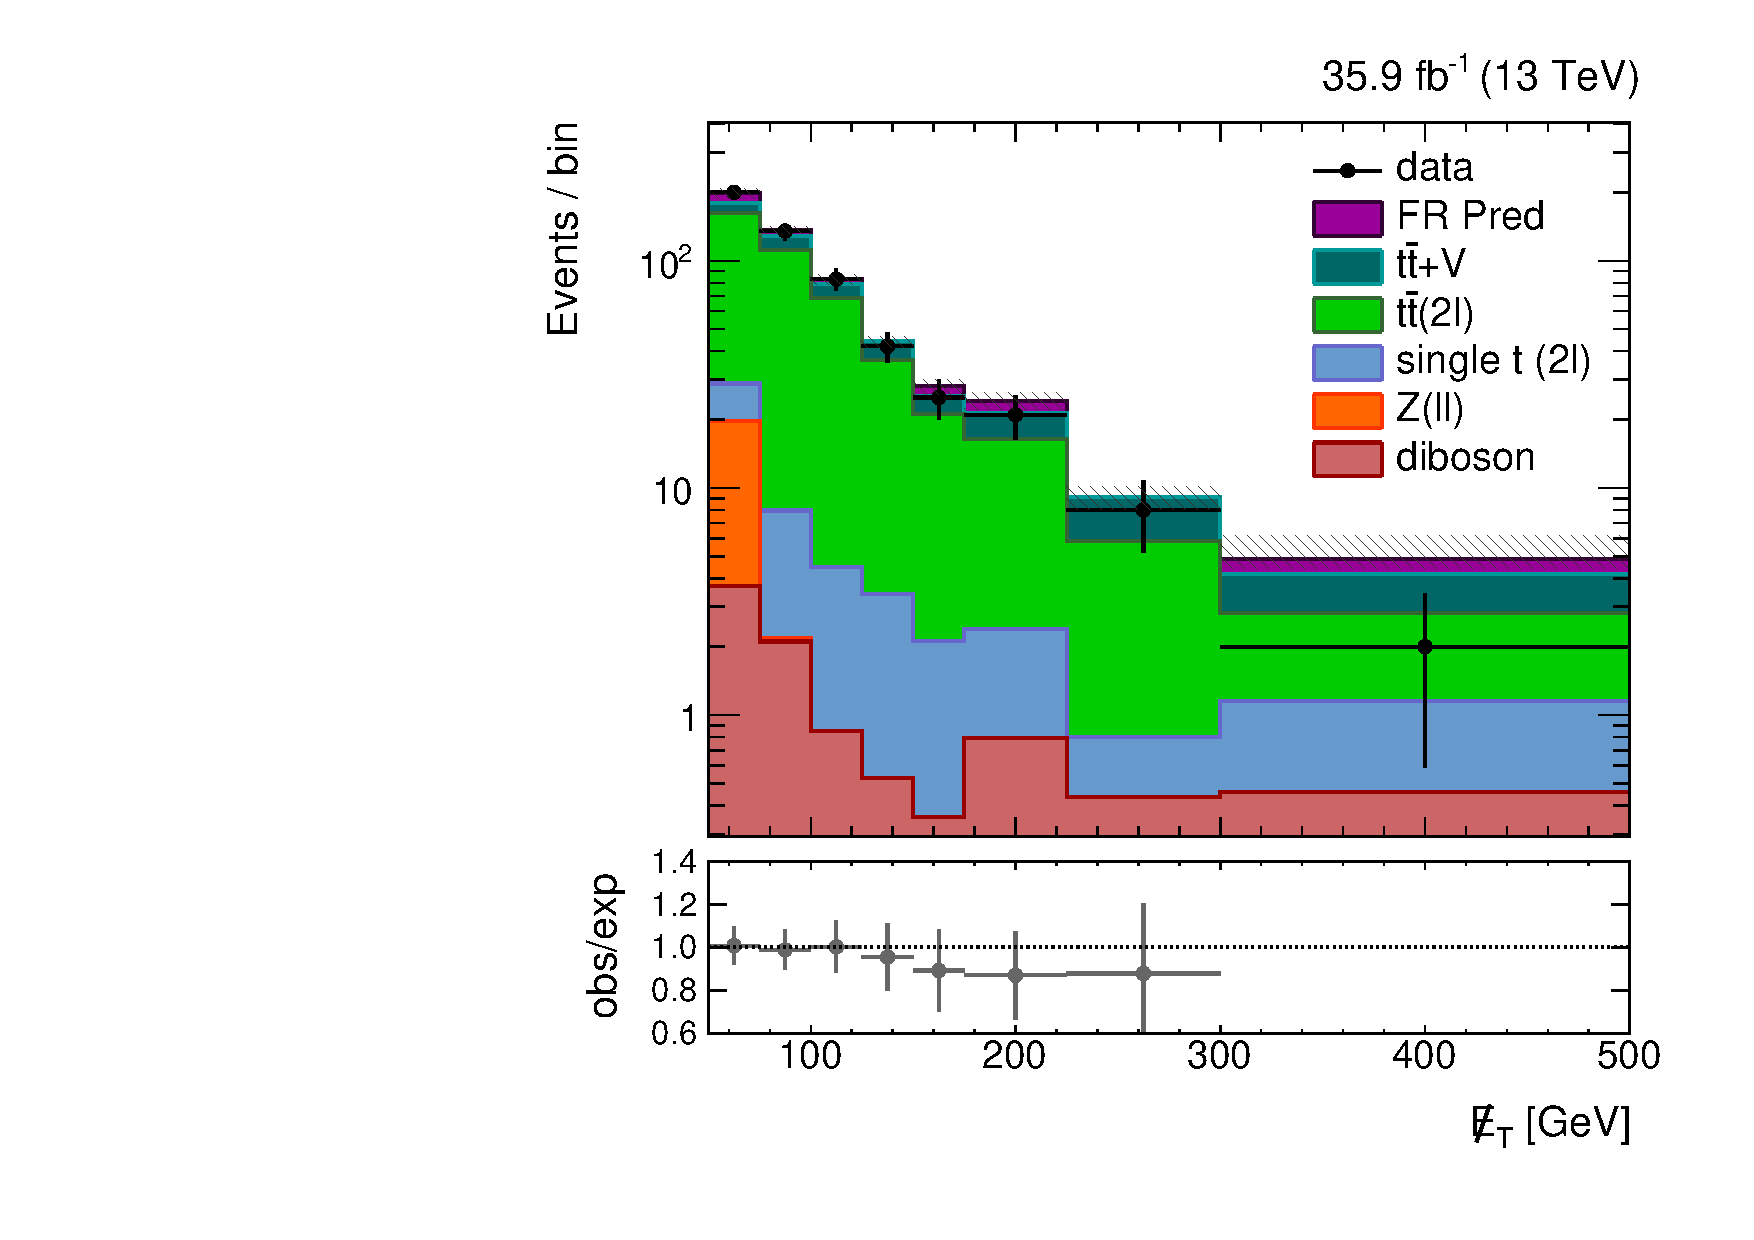
\includegraphics[width=0.32\textwidth]{figs/met_close_ee.pdf}}
  \subfloat[][$e\mu$ channel]  {\label{subfig:fr_close_em}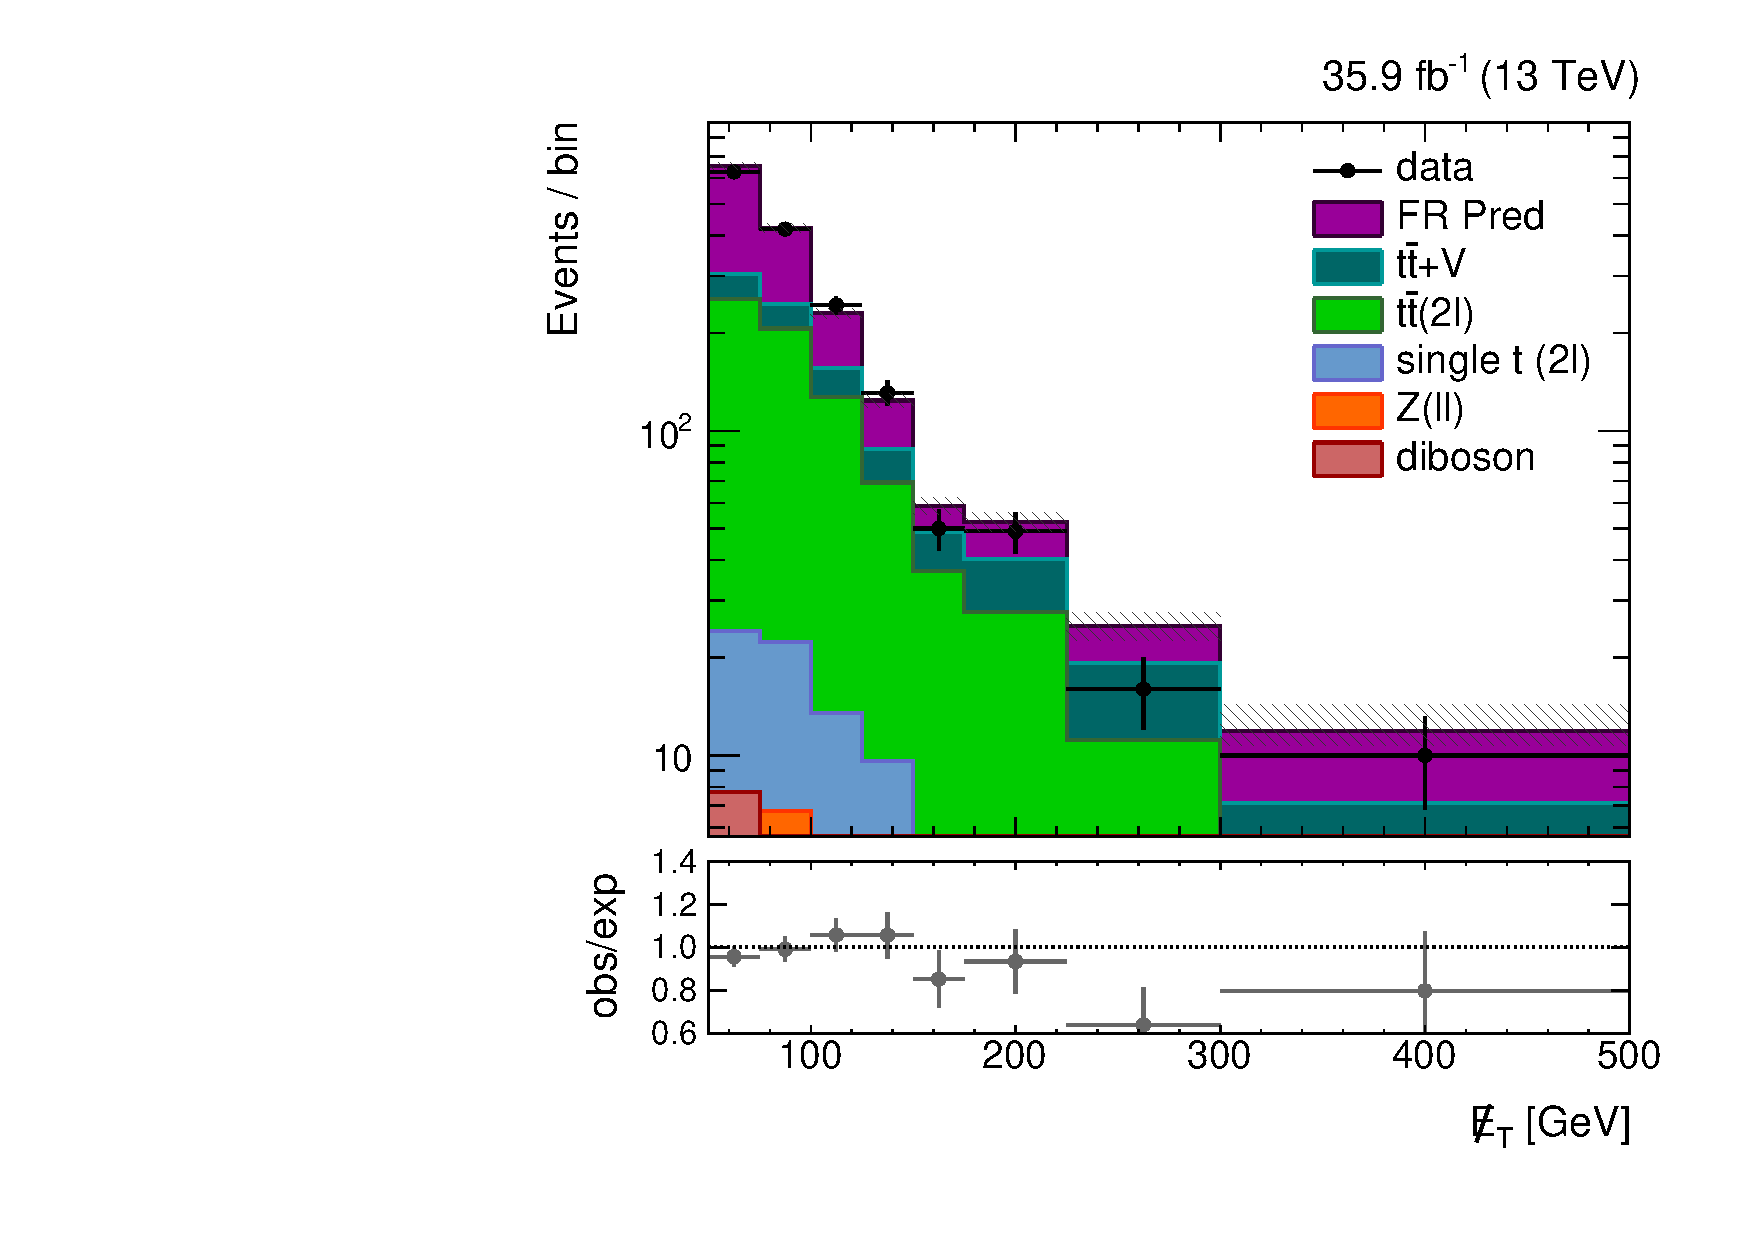
\includegraphics[width=0.32\textwidth]{figs/met_close_em.pdf}}
  \subfloat[][$\mu\mu$ channel]{\label{subfig:fr_close_mm}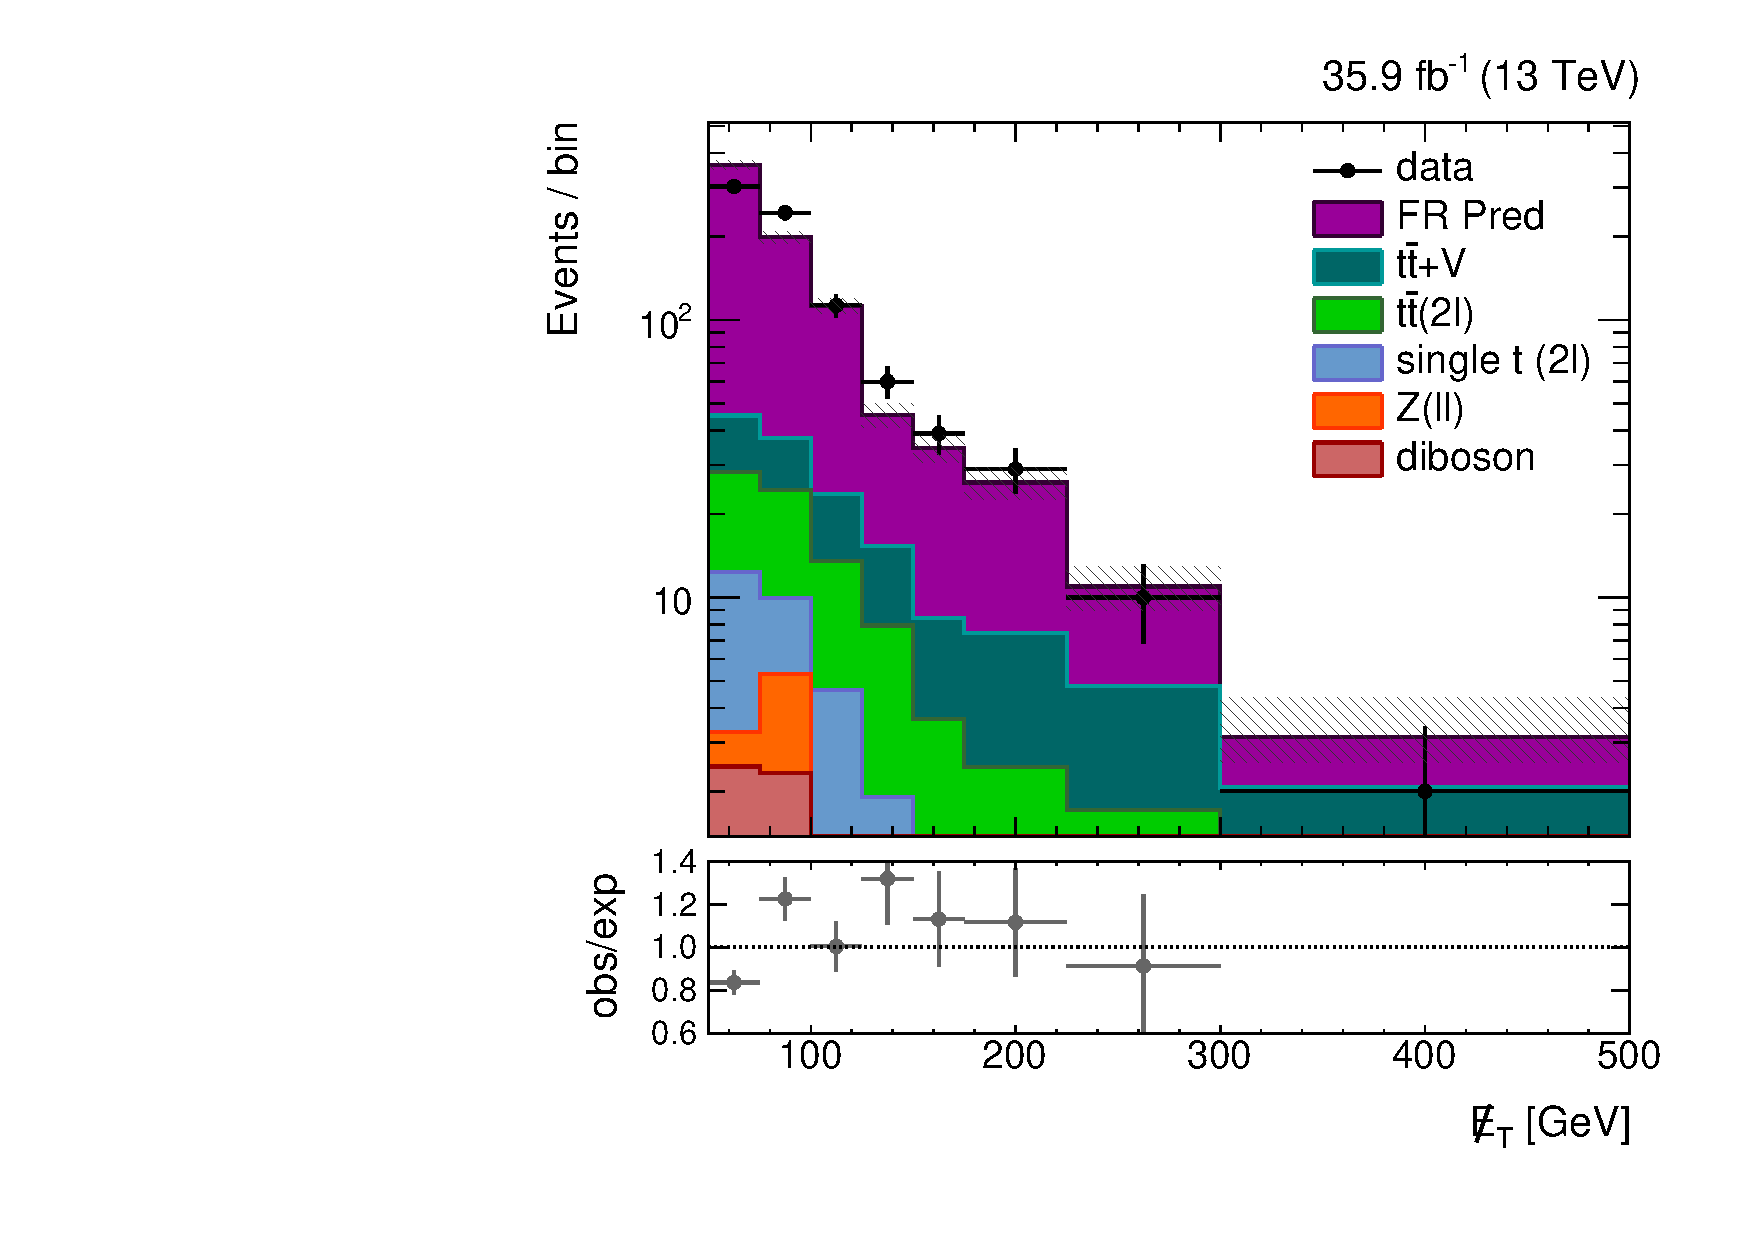
\includegraphics[width=0.32\textwidth]{figs/met_close_mm.pdf}}
  \caption{The \ptmiss distributions in the fake rate method validation region. All expected backgrounds are estimated using simulation, except for the fake lepton contribution, denoted ``FR Pred'' which is estimated via the fake rate method.}
  \label{fig:fr_close}
  \end{center}
\end{figure}
